% --------------------------------------------------------------
% This is all preamble stuff that you don't have to worry about.
% Head down to where it says "Start here"
% --------------------------------------------------------------
\documentclass[11pt]{article}

%\documentclass[12pt]{article}
 
\usepackage[margin=1.5in]{geometry} 
\usepackage{amsmath,amsthm,amssymb}
\usepackage[T1]{fontenc} 
\usepackage[utf8]{inputenc}
\usepackage{lmodern}
\usepackage{graphicx}
\usepackage{indentfirst}
\graphicspath{ {images/} }
\usepackage[compact]{titlesec}
\usepackage{hyperref}
\usepackage{chngcntr}
\usepackage{lineno}
\usepackage{caption}
\usepackage{subcaption}
 \usepackage[dvipsnames]{xcolor}
\newcommand{\N}{\mathbb{N}}
\newcommand{\Z}{\mathbb{Z}}
 
% \newenvironment{theorem}[2][Theorem]{\begin{trivlist}
% \item[\hskip \labelsep {\bfseries #1}\hskip \labelsep {\bfseries #2.}]}{\end{trivlist}}
% \newenvironment{lemma}[2][Lemma]{\begin{trivlist}
% \item[\hskip \labelsep {\bfseries #1}\hskip \labelsep {\bfseries #2.}]}{\end{trivlist}}
% \newenvironment{exercise}[2][Exercise]{\begin{trivlist}
% \item[\hskip \labelsep {\bfseries #1}\hskip \labelsep {\bfseries #2.}]}{\end{trivlist}}
% \newenvironment{problem}[2][Problem]{\begin{trivlist}
% \item[\hskip \labelsep {\bfseries #1}\hskip \labelsep {\bfseries #2.}]}{\end{trivlist}}
% \newenvironment{question}[2][Question]{\begin{trivlist}
% \item[\hskip \labelsep {\bfseries #1}\hskip \labelsep {\bfseries #2.}]}{\end{trivlist}}
% \newenvironment{corollary}[2][Corollary]{\begin{trivlist}
% \item[\hskip \labelsep {\bfseries #1}\hskip \labelsep {\bfseries #2.}]}{\end{trivlist}}

% \newenvironment{solution}{\begin{proof}[Solution]}{\end{proof}}
% \newcommand*\mean[1]{\bar{#1}}

\counterwithin{equation}{section}
\counterwithin{equation}{subsection}

\begin{document}

\begin{titlepage}
\begin{center}

% 1. The title of the thesis/dissertation, centered 2Ó below the top of the page

\vspace{2in}
\Large \bf
The Diverse and Dynamic Nature of Mixtures in Active Matter Systems


% 2. Your name, centered 1Ó below the title.
\vspace{61pt} % 1 in = 72pt, 11pt for the line with text
\large Nicholas Jacob Lauersdorf
\end{center}


%3. The following statement, within the full mar- gins, 1Ó below your name:
%ÒA dissertation [or thesis] submitted to the faculty of the University of North Carolina at Chapel Hill in partial fulfillment of the requirements for the degree of	in the Department [or School or Curriculum] of      .Ó

\vspace{50pt}
\noindent \large
A literature review submitted to the faculty of the University of North Carolina at Chapel Hill
in partial fulfillment of the requirements for the degree of Doctor of Philosophy in
the Applied Physical Sciences department in the College of Arts \& Sciences.


%4. On the lower half of the page, centered, the words ÒChapel HillÓ
%and one line below that, the year in which your committee approves
%the completed thesis/dissertation.
\vspace{50pt}
\begin{center}
\large
Chapel Hill\\
2020
\end{center}

%5. On the right-hand side of the page, ÒApproved by,Ó followed by lines for the
%signatures of the adviser and four (two for thesis) readers. List

\vfill
\begin{flushright}
\begin{minipage}[t]{1.5in} \large
%Approved by:\\
To be approved by: \\
Daphne Klotsa \\
Ed Samulski \\
Ehssan Nazockdast \\
Greg Forest \\
Rene Lopez \\
Zhiyue Lu
\end{minipage}
\end{flushright}

\end{titlepage}

%\title{%
%  Kinetic theory and liquid phase density from pair-force in active Brownian particles \\
%  \large Derivation and resulting expressions}
%\author{Nicholas J. Lauersdorf}

%\maketitle

\section{Introduction}
\label{S:1}
Active matter encompasses systems that consist of a large number of self-propelled motile agents that convert local energy into motion. As a result, the system is dynamic and continuously driven out of equilibrium.  Active matter is most commonly seen in biological systems, such as motor proteins which convert ATP into motion in order to assemble mitotic spindles \cite{Schliwa, Oriola}, algae propelled by flagella \cite{Drescher}, and bacteria with either density-dependent \cite{Zhang} or other forms of motility \cite{Peruani}.  Not only is active matter observable on the micro-scale, but it is clearly visible to the naked eye in every day sights, such as flocking in birds \cite{Ballerini}, schooling of fish  \cite{Lopez}, and the organization of ants into rafts to survive a flood \cite{Mlot} or a ladder to reach a food supply \cite{Hu} [Figure \ref{fig:ActiveMatter}]. These are all extremely different organisms with varying forms of locomotion, but their independent motion can lead to unique, collective behavior to achieve a common goal \cite{Zohdi}.  

\begin{figure}[ht]
\centering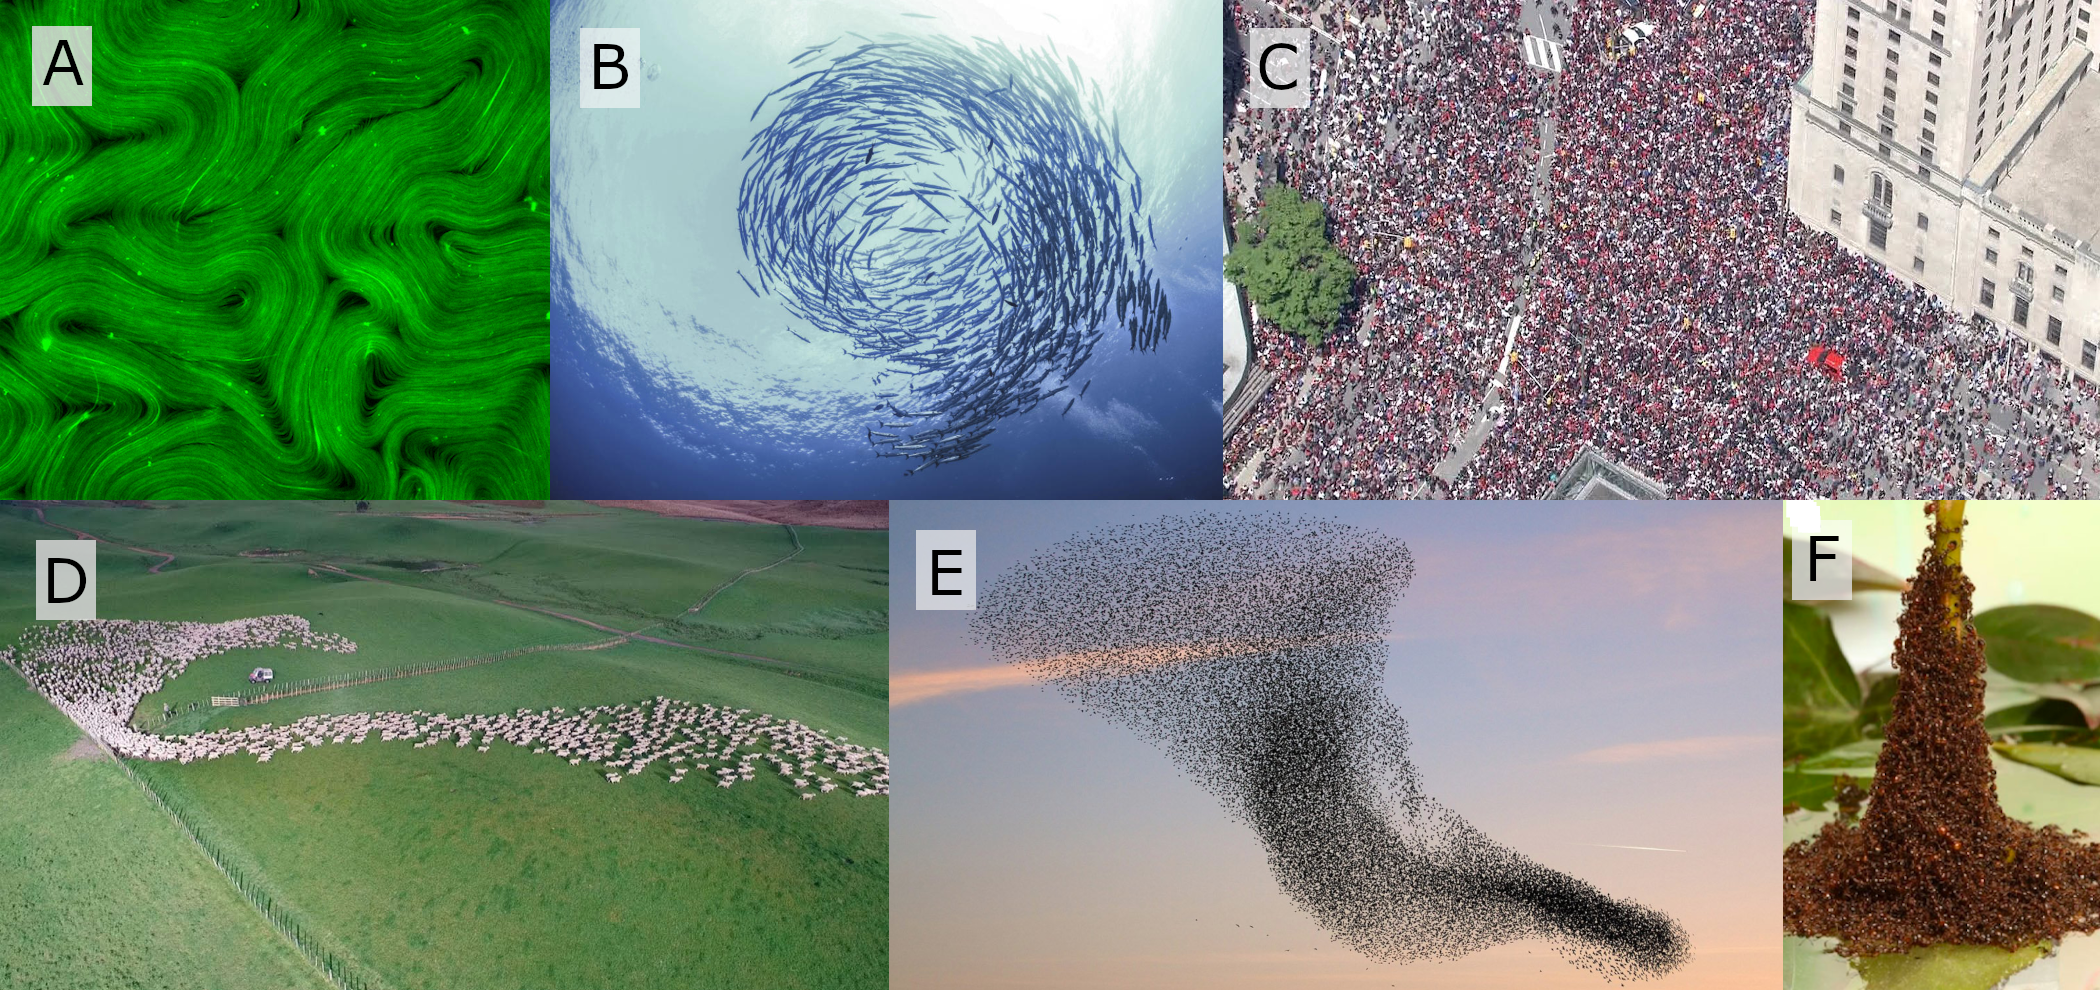
\includegraphics[width=1.0\linewidth]{Untitled.png}
\caption{Common active matter systems, such as A) active nematic fluids, B) schools of fish, C) human crowds, D) a sheepdog herding sheep, E) Flocking of starling, and F) an ant colony forming a ladder to reach food \cite{Hu}.}
\label{fig:ActiveMatter}
\end{figure}

Dynamic, collective phenomena, such as swarming \cite{Vicsek, Romanczuk}, clustering \cite{Peruani2, Wensink, Yang7}, and active swirling \cite{Aranson, Drescher2}, commonly occur across active matter in systems of only a single species. However, diversity is omnipresent in nature and, in turn, a wide array of active systems, taking the form of mixtures.  The prevalence of inhomogeneous mixtures in nature raises the question of what  would happen if we were to consider a heterogeneous active mixture, for example by introducing a second, predatory species. Bird flocks demonstrate highly variable flocking patterns that are contingent on whether they are intended for traveling or avoiding predators.  The commonly seen `V' flock shape during travel is a rather simple shape, but when a predatory hawk is introduced, the birds move seemingly randomly yet together [Figure \ref{fig:ActiveMatter}E].  Similar to the `V' shape flock, birds still prefer to fly oriented with each other.  Although, while in this dense flock, each bird can only see as far as its nearest few neighbors, giving rise to a short-range local interaction that determines each bird's orientation.  Due to this short-range interaction, each individual's motion contributes to its neighbors who in turn influence their neighbors and so on.  These local interactions give rise to global order: a dynamic, cluster of birds that collectively respond to the individual motion of the hawk.  These new and unique behaviors that arise with multivariable mixtures motivate us to continuously evolve our research to increasingly more complex systems that will eventually represent the complexities in natural systems.

\subsection{Active Mixtures}

Active mixtures serve as a common aspect of everyday life whether it is a sheepdog herding a flock of sheep, humans in a crowd simply moving at different speeds, or a colloidal dispersion of various shapes and sizes.  These realistic mixtures are incredibly inhomogeneous, obscuring the influence of each variable on their already complex behavior. For this reason, characterizing multivariable systems must be a systematic process. Our ancestors did not go directly from making simple iron bars to the 10-component alloy steel of the modern age. Similar to the evolution of metallurgy, we must take a step-by-step approach to gradually increase complexity as we begin to characterize the role of each component.  Therefore, binary mixtures, such as two species of fast and slow particles, are the next most logical step in expanding our understanding from monodisperse model systems to the heterogeneous mixtures seen in nature.

Though the complexity of these mixed, active systems is great, the potential benefit of understanding them is apparent in active colloidal dispersions.  These mixed colloidals systems display the same uniqueness of clustering as their monodisperse counterparts while adding even more diverse capabilities like activity induced transport \cite{Ghosh}, sorting \cite{Chen5}, enhanced crystallization \cite{Meer}, reduced degree of sedimentation \cite{Palacci4}, and even more unique and enhanced phase separation behavior \cite{Kolb}.  The aforementioned capabilities could serve to enhance many pre-existing technologies, such as increased crystallinity in optoelectronic devices \cite{Meer, Castro}, reduced sedimentation rate in cements \cite{Palacci4}, drug delivery and targeting without an expensive, external field \cite{Ghosh6}, in-vivo tissue generation \cite{Patterson}, and superior performing robotic swarms for industrial applications \cite{Brambilla}.  Though its practical application in a variety of fields may be far off, characterizing and understanding each variable in these complicated, mixed systems is the next big step in enabling the development of this concept into useful applications.

 The focus of this thesis is to understand active mixtures but in order to understand mixtures, one must first understand the underlying physics of monodisperse systems. In this thesis, we have gone through, step-by-step in increasing complexity, to build the idea that monodisperse systems are mere case studies of their more complex, mixed counterparts. We first introduce commonly used models in the active matter field, such as the Vicsek model [Section \ref{VicsekModel}], the run-and-tumble particle [Section \ref{RTPmodel}], and the active Brownian particle [Section \ref{ABPsyo}], our system of interest. In order to see some semblance of clarity, we start with very basic, one-variable systems (i.e. monodisperse passive Brownian systems [Section \ref{passiveparticlesystem}]) and continually expand to greater complexities to understand the interplay of components, such as activity [Sections \ref{ABPactivity}, \ref{monodisperseABPactivity}, \ref{activepassiveABPactivity}, and \ref{activeactiveABPactivity}], activity mechanisms [Section \ref{propulsionmech}], non-steric interparticle forces [Section \ref{interactionmech}], softness [Section \ref{softnessmix}], and shape/size [Section \ref{shapessizes}] within these multi-variable systems.  As is evident, the properties of these active mixtures are only beginning to be understood with fundamental questions still looming, such as what exactly is equilibrating in these steady-state clusters?  

\section{Active Matter Models}

Though these active systems are widely varying from birds to nanoscale particles, comparable system-wide behavior arises. Collective behavior arises despite the large variance in length scale, dependent mostly on self-propulsion and interaction mechanisms. As a result, this brings hope that similarly behaving active matter can be physically quantified into a simple, predictive model.  Though there are many more complex active systems, in this section, we will describe the three simplest cases of active matter: the Vicsek model, the Run-and-Tumble Particle (RTP), and the active Brownian particle (ABP). We see that these active matter species and their respective behavior vary starkly in terms of their re-orientation mechanism.  The Vicsek model accounts for locally-aligning species, such as flocks of birds.  RTPs, go through periods of linear motion followed by instantaneous, random re-orientations.  Bacteria propelled by flagella most commonly display this mechanism of motion.  The last and most important model for the purpose of this thesis is the ABP in which self-propelled colloids continuously rotate through thermal noise as they propel themselves through a medium.

Besides simply deepening our understanding of the underlying physics, these models serve to enable development of active materials for human use.  Of great interest is the capability to use synthetic self-propelled colloidal particles, encompassed in the ABP model, for medical and engineering purposes, such as drug delivery and targeting \cite{Li, Orozco}, environmental remediation through neutralization of contaminants \cite{Gao2, Li3}, and rapid medical diagnoses via motility-enhanced reactions in chemical testing \cite{Garcia, Perez}.  In order to develop these materials to the best of our ability, we must first characterize the properties of ABPs and how they are influential to the system's behavior. 

\subsection{Vicsek Model}\label{VicsekModel}

The Vicsek model, intended to simulate the motion of flocking birds, is one of the simplest models to demonstrate particle alignment and clustering in an active system \cite{Vicsek}.  Each particle moves with constant speed, dictating its position ($\boldsymbol{r}$) at the next discrete time step \cite{Ginelli}:

\begin{equation}\label{deflection}
    \boldsymbol{r}_\text{i}^{\text{t}+\Delta\text{t}} = \boldsymbol{r}_{\text{i}}^{\text{t}} + \Delta t v_0 
    \boldsymbol{s}_{\text{i}}^{\text{t} + \Delta\text{t}}
\end{equation}

\noindent where the orientation ($\boldsymbol{s}$) and preferred speed ($v_0$) coincides with the velocity ($\boldsymbol{v}=v_0 \boldsymbol{s}$).
At each time step ($\Delta\text{t}$), each particle synchronously reorients itself to the average orientation of its neighbors within a local vicinity [Figure \ref{fig:Vicsek}].  The orientation also experiences a thermal white noise perturbation ($\xi_\text{i}^\text{t}$) that is delta-correlated ($\langle\xi_\text{i}^\text{t}\xi_\text{j}^\text{k}\rangle \sim \delta_{\text{tk}}\delta_{\text{ij}}$) and time averages to 0 ($\langle\xi_\text{i}^\text{t}\rangle = 0$). These two terms result in the following rotation per time step  \cite{Ginelli}:

\begin{equation}\label{rot}
    \theta_\text{i}^{\text{t}+\Delta\text{t}}=\text{Arg}\left[\sum_j n_{\text{ij}}^\text{t}\boldsymbol{s}_\text{j}^\text{t}\right]+\eta\xi_\text{i}^\text{t}
\end{equation}

The orientation, $\boldsymbol{s}=(\text{cos}\theta,\text{sin}\theta)$, depends on the average direction of all particles within a neighborhood $S_\text{i}$ of radius $R_0$ around the $\text{i}^\text{th}$ particle.  Arg returns the angle corresponding to the average vector $\sum_j n_{\text{ij}}^\text{t}\boldsymbol{s}_\text{j}^\text{t}$. $n_{\text{ij}}^\text{t}$ is the connectivity matrix to determine neighboring particles, which is defined as \cite{Ginelli}:

\begin{equation}\label{conn}
  n_{\text{ij}}^\text{t}=\begin{cases}
    1, & \text{if $|\boldsymbol{r}_\text{i}^\text{t}-\boldsymbol{r}_\text{j}^\text{t}|<R_0$}.\\
    0, & \text{if $|\boldsymbol{r}_\text{i}^\text{t}-\boldsymbol{r}_\text{j}^\text{t}|>R_0$}.
  \end{cases}
\end{equation}


\begin{figure}[ht]
\centering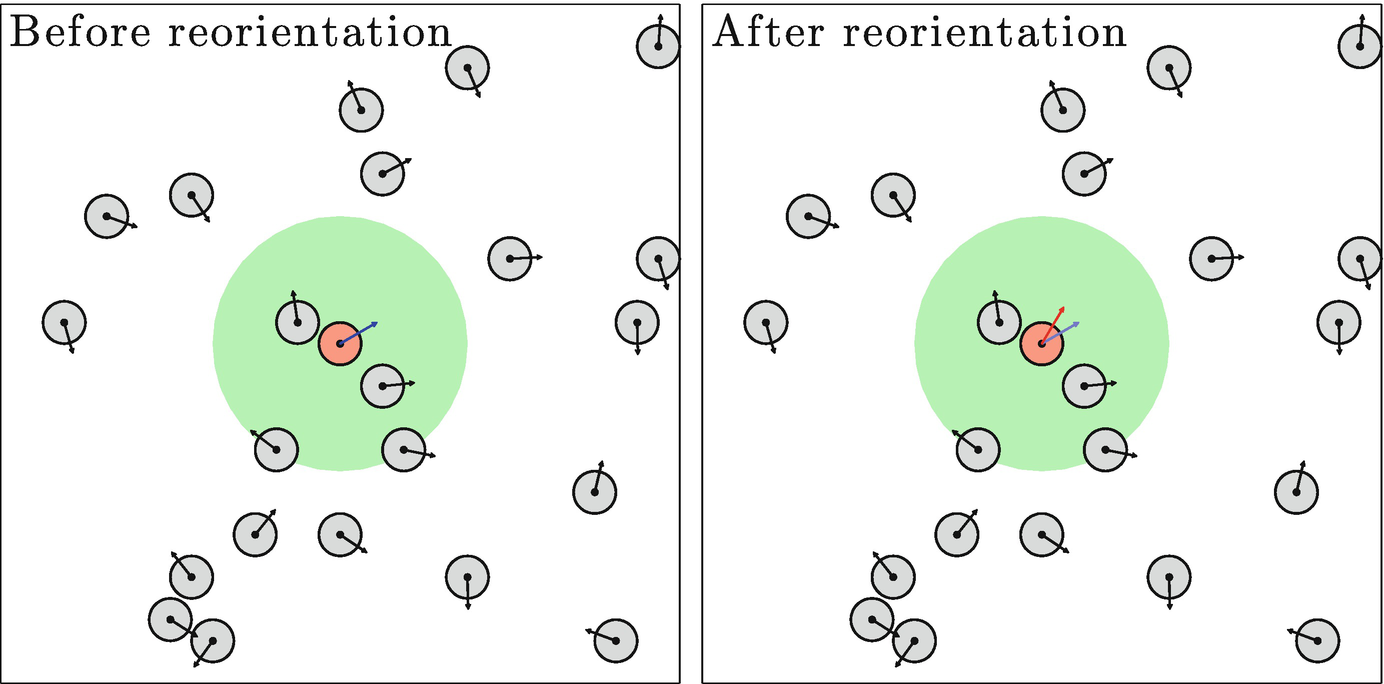
\includegraphics[width=0.8\linewidth]{462743_1_En_7_Fig6_HTML.png}
\caption{Vicsek model: Current and proceeding orientation visible in blue and red respectively.  The average orientation is determined within the flocking radius (green area) for the current time step.  \cite{Toschi}}
\label{fig:Vicsek}
\end{figure}

At sufficient system particle fraction, the system goes through a phase transition from a  disordered state into aligned synchronized flocks. Due to interparticle interactions only within its immediate vicinity, the phases are locally ordered but generically correlated over long range \cite{Mahault}.  When subject to long-range interactions or some incompressibility condition, universal order can occur over sufficient time \cite{Kayal}.  

\subsection{Run-and-tumble Particle Model}\label{RTPmodel}

Run-and-tumble motion is prevalent in biological systems like Eschererichia coli microswimmers \cite{Sidortsov, Watari}.  When flagella are all rotating in the same direction, they work together and the bacterium runs in a constant direction at a preferred swim speed. Run-and-tumble particles (RTPs) swim in a linear motion until a 'tumble' event happens, occurring at a random rate, where their orientation is instantaneously reassigned to a random direction [Figure \ref{fig:rtp}].  The self-induced tumble occurs when the flagella motion becomes suddenly uncoordinated and the flagella work against each other, causing a random reorientation for its next run event. Though the direction cannot be controlled, the reorientation frequency can be changed such that the bacterium stochastically migrates towards a preferred environment, such as in a temperature gradient or a concentration gradient of a molecule of interest \cite{Berg, Berg2}.  The overall motion of RTPs embodies an enhanced diffusion over purely thermal rotation, enabling a greater ability for the bacterium to explore its environment.

\begin{figure}[ht]
\centering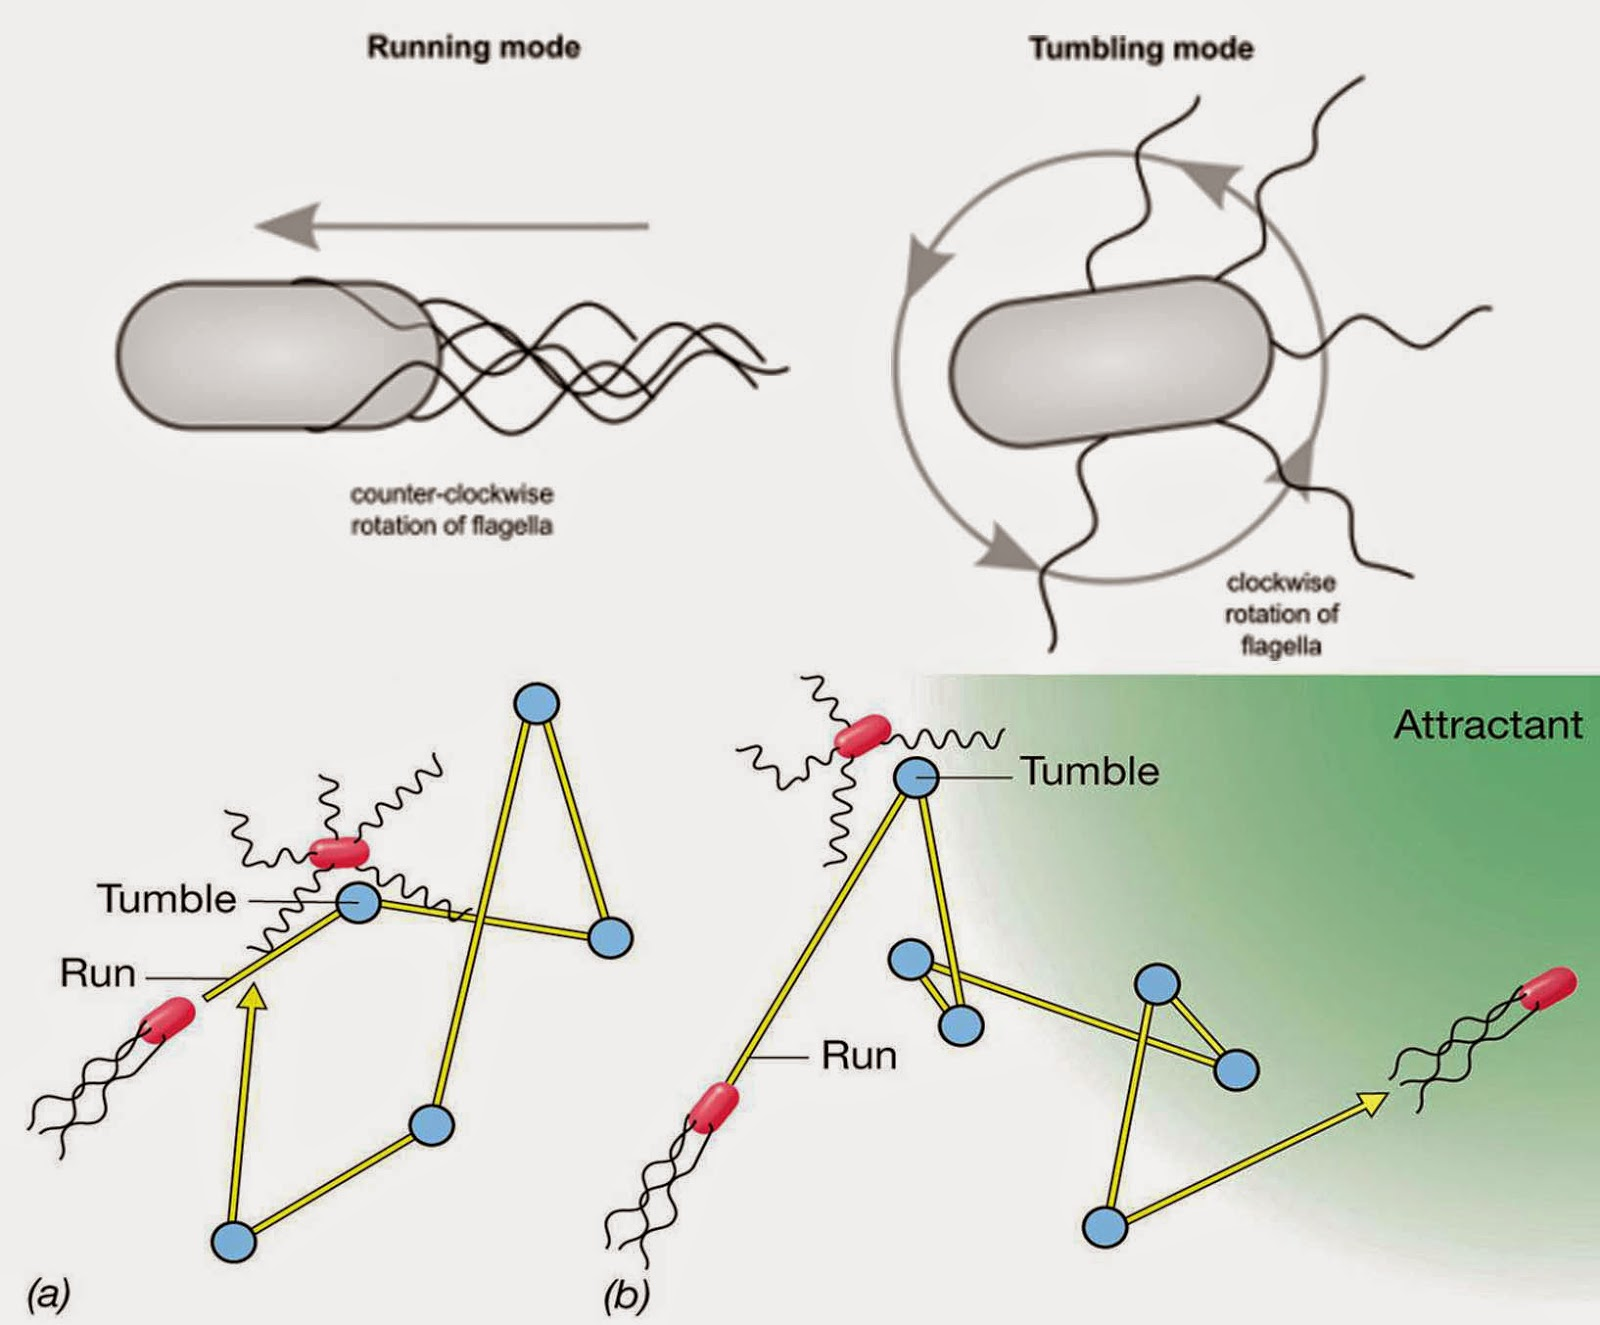
\includegraphics[width=0.8\linewidth]{2-run.jpg}
\caption{Run-and-tumble mechanism (top) and RTP motion over short time scales (bottom). On the bottom left, the motion is random; whereas, the bottom right shows preferential motion due to it entering the local vicinity (green) of an 'attractive' force, such as food.}
\label{fig:rtp}
\end{figure}

Mathematically, the tumble motion is usually described in terms of two random variables: the tumble angle ($\Psi_\text{T}$) and the tumble time ($\text{t}_\text{T}$) [Figure \ref{fig:rtpangle}]. The tumble angle is the angle between the orientation at the end of a run and the start of the following run. For mathematical simplicity, the tumble deflection ($\text{x}_\text{T}=\text{cos}(\Psi_\text{T})$ with $|\Psi_\text{T}|\le\pi$) is typically the parameter used to define the Langevin equation of tumble motion \cite{Fier2}:

\begin{equation}\label{deflection2}
    \dot{\text{x}} = -\frac{\text{dU}}{\text{dx}}+\eta(\text{t})
\end{equation}

\noindent where $\eta(\text{t})$ is an additive Gaussian white noise term which averages to zero in time ($\langle\eta(\text{t})\rangle=0$) and is correlated in time by: $\langle\eta(\text{t})\eta(\text{t}')\rangle=2\text{D}\delta\delta(\text{t}-\text{t}')$ where D is the noise intensity.  $\text{U}=\text{U}(\text{x})$ is a potential that has been derived from experimental measurements of the tumble angle ($\Psi_\text{T}$) distribution \cite{Fier}:

\begin{equation}\label{potential}
    \text{U}(\text{x}) = \text{U}_{0}-\rho\left[\text{x}-\frac{\gamma}{\delta}\text{cosh}(\delta \text{x})\right]
\end{equation}

\noindent where $\text{U}_{0}$ is an adjustable constant.  $\delta$, $\gamma$, and $\rho$ are three constants linked together by the following relationship: 

\begin{equation}\label{relation}
    \rho^2\delta\sqrt{1+\gamma^2}=\text{C}=\text{constant}
\end{equation}

\noindent The relationship of $\delta$, $\gamma$, and $\rho$ specify whether the system is in the movement state of either a run ($\rho(\delta_\text{R},\gamma_\text{R})=\text{r}>1$) or tumble ($\rho(\delta_\text{T},\gamma_\text{T})=1$). For reference, $\delta_\text{T}=9.062$ and $\gamma_\text{T}=6.63 \text{x} 10^{-3}$ correspond to the tumble motion, and $\delta_\text{R}=4.71 \text{x} 10^{-2}$ and $\gamma_\text{R}=4.98$ correspond to the run motion.  Using eqn. \ref{relation}, we find that $\text{C}\approx \delta_\text{T}$ and the ratio $\text{r}\approx\sqrt{\delta_\text{T}/(\delta_\text{R}\gamma_\text{R})}\approx6.21$, approximately agreeing with the experimentally measured ratio of $\text{r}_{\text{exp}}\approx6.14$ for E. coli \cite{Berg5}.

\begin{figure}[ht]
\centering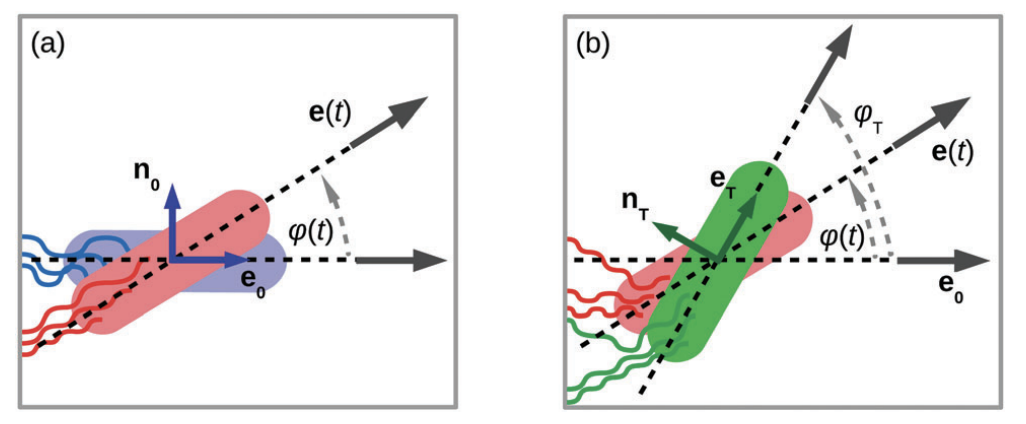
\includegraphics[width=0.8\linewidth]{Screen Shot 2020-09-18 at 3.21.13 PM.png}
\caption{a): $\boldsymbol{e}(t)$ represents the current orientation of the bacterium. $\Psi(t)$ represents the angle between $\boldsymbol{e}(t)$ and the incoming direction $\boldsymbol{e}(t_0)$. b): $\boldsymbol{e}(t_\text{T})$ is the resulting outgoing bacteria direction with total tumble angle of $\Psi(t_\text{T})$ after the total tumble time of $t_\text{T}$.  $\boldsymbol{e}(t)$ and $\Psi(t)$ still represent the orientation and rotation angle at the current time t still \cite{Fier2}}
\label{fig:rtpangle}
\end{figure}

\subsection{Active Brownian Particle Model}\label{ABPsyo}

From solution fabricated solar cells to cement and even to the lifeblood of Wisconsin, milk, colloidal dispersions are utilized in a wide array of scientific research and commercial products.  These colloidal solutions do not compare in function, but their physics is fairly akin as can be seen by their equations of motion.  A colloidal dispersion consists of nanoscale particles suspended in a solvent of smaller particles. In the aforementioned systems, these colloidal particles are completely passive.  However, it is also possible for colloidal systems to consist of self-propelling particles. 

A well-studied, experimental self-propelling particle is the catalytic Janus particle [Figure \ref{fig:janus}]. In the case of active Janus particles, one side of the Janus particle is a catalyst that interacts with the solution while the other side is inert and does not, resulting in a net force and, in turn, propulsion.  Different chemical reactions continuously occur on the catalyst surface, leading to a local gradient of either solute concentration, electric potential, or temperature that induces motion via self-diffusiophoretic \cite{Howse, Golestanian, Popescu}, self-electrophoretic \cite{Moran, Moran2, Ebbens, Brown, Brown2}, or self-thermophoretic \cite{Yang, Jiang, Samin} propulsion mechanisms respectively.   

\begin{figure}[ht]
\centering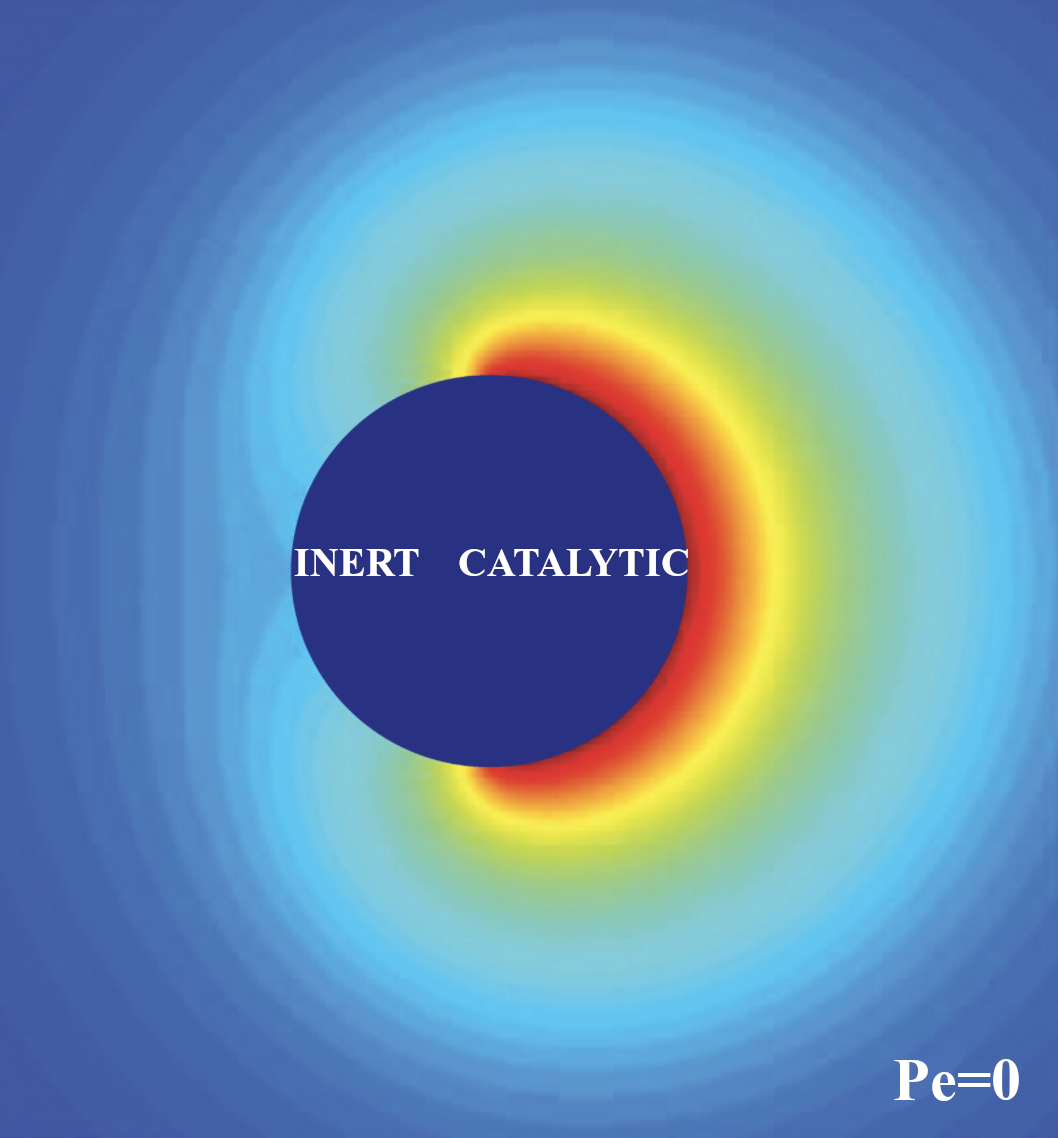
\includegraphics[width=0.5\linewidth]{Screen Shot 2020-08-05 at 8.17.05 PM2.png}
\caption{ Concentration of reactant species (red represents low concentration; blue represents the far-field concentration) near a self-diffusiophoretic Janus particle. The catalytic half consumes reactant particles. A repulsive force to the right is being exerted onto the swimmer by the greater reactant concentration near the inert side, propelling the particle to the right \cite{Moran}.}
\label{fig:janus}
\end{figure}

Despite different self-propulsion mechanisms, the extent of displacement depends strictly on the intrinsic swim speed [Figure \ref{fig:displacement}] in addition to the reorientation rate, enabling one to quantify the activity in a single term, the P\'{e}clet number, for Stokesian agents:

\begin{equation}\label{Pe}
    Pe = \frac{3v_{\text{p}}\tau_{\text{r}}}{\sigma}
\end{equation}

\noindent Where $\tau_{\text{r}}$ is the reorientation time.  As on can see from eqn.~\ref{Pe}, a continuum of activities is introduced to explore. The following sections will start with the simplest case, passive particles ($Pe=0$) and build upon this knowledge in increasing complexity to introduce active particles ($Pe>0$).



\subsubsection{The Passive Brownian Particle}\label{passiveparticlesystem}

 In most colloidal dispersions, colloidal particles are passive, i.e. they are undergoing Brownian motion. In general, their motion is exclusively determined by means not of their own, whether it is motion due to other particles, the fluid, or an external field whose force is the source of motion (i.e. magnetic attraction) as opposed to inducing a particle's self-generated locomotion mechanism.  
 
 Particles can interact through either short-range or long-range interaction mechanisms ($\boldsymbol{F}_{\text{C}}$).  We will consider the simplest case which is colloidal particles that interact through short-range steric repulsive forces, where particles physically repel each other once they begin to touch or overlap via a collision (excluded volume).  In Monte Carlo simulations, a strict hard sphere approach is possible, but, in molecular dynamics, the best approximation of this hard-sphere repulsion is a steep Weeks-Chandler-Andersen (WCA) potential [Figure \ref{fig:WCA}]:
 
\begin{equation}\label{LJ}
  U(r_{\text{i,j}})=\begin{cases}
    4\epsilon\left[\left(\frac{\sigma}{r_{\text{i,j}}}\right)^{{12}}-\left(\frac{\sigma}{r_{\text{i,j}}}\right)^6\right]+\epsilon, & \text{if $0\leq r_\text{i,j} \leq r_\text{cut}$}.\\
    0, & \text{if $r_\text{i,j}>r_\text{cut}$}.
  \end{cases}
\end{equation}
 
\noindent with corresponding force:
 
 \begin{equation}\label{LJForce}
  F_{\text{WCA}}(r_{\text{i,j}}\le r_{\text{cut}}) =
    \frac{24\epsilon}{\sigma}\left[2\left(\frac{\sigma}{r_{\text{i,j}}}\right)^{13}-\left(\frac{\sigma}{r_{\text{i,j}}}\right)^7\right]
\end{equation}

 \noindent where each $i^{\text{th}}$ and $j^{\text{th}}$ particle repel each other when their separation distance, $r_{\text{i,j}}$, is less than the separation limit ($r_{\text{cut}}=2^{1/6}\sigma$). The depth ($\epsilon$) determines the strength of the repulsion and, in turn, the allowed particle overlap and softness \cite{Kolb}. For maximum particle rigidity, we find an interaction strength of \cite{Kolb}:

\begin{equation}\label{HardEpsmono}
  \epsilon_\text{hard} =
    \left[\frac{4F_{\text{A}}}{24}+10\right]k_\text{B}T
\end{equation}

\noindent where $\boldsymbol{F}_{\text{A}}$ is the active force of each particle.  In a purely passive system, $\boldsymbol{F}_{\text{A}}=0$, such that  $\epsilon_{\text{hard}}\rightarrow10k_\text{B}T$. $\epsilon<\epsilon_{\text{hard}}$ represents a soft sphere system with decreasing steepness in $\boldsymbol{F}_{\text{WCA}}$ as $\epsilon\rightarrow0$ [Figure \ref{fig:WCA}]. Though this literature review will focus on active Brownian particles interacting solely through volume-exclusion reactions, other interparticle forces can exist, such as orientational alignment, as seen in the Vicsek model \cite{Vicsek}, or dipolar ineractions \cite{Goyal, Maloney}.

\begin{figure}[ht]
\centering\includegraphics[width=0.65\linewidth]{download (29).png}
\caption{Potential strength ($u_\text{ij}$) of the WCA potential versus the distance from a particle's center of mass ($r_\text{i,j}$) normalized by the particle's uncompressed diameter ($\sigma$).  The WCA potential corresponding to a hard sphere (dashed line) and soft sphere (solid line) of softness $\epsilon=0.1$ are shown.}
\label{fig:WCA}
\end{figure}

Even though the WCA potential is a purely repulsive force, a dense, highly ordered phase can still form. An increase in visible order, such as a crystalline lattice, can be associated with an increase in microscopic disorder.  This concept leads to many counter-intuitive phenomena such as entropy driven crystallization and phase separation. As a system becomes more crystalline, it is generally thought to be more ordered, i.e. liquids are thought to be 'disordered' whereas crystalline solids are highly 'ordered'.  If this were true, Boltzmann's expression for entropy ($S=k_\text{B}ln\Omega$) would suggest that the transition from the liquid to the crystalline phases is solely energy-driven, requiring a decrease in temperature to offset the decrease in entropy. However, many crystallization processes may actually be entropy-driven.  


As density increases, the free-volume per particle in the ordered, phase-separated state continuously increases above that of the disordered state, leading to the phase-separated state having greater entropy and, in turn, entropy-driven phase separation \cite{Frenkel2}.  At system packing fractions greater than some critical value, the entropy of the ordered state becomes greater than that of the disordered state, leading to entropy-driven hard-sphere crystallization.  On the other hand, hard sphere crystallization can also occur in systems with lower system packing fraction than the critical value. A local packing fraction greater than the critical packing fraction can be induced upon the addition of a strong enough attractive interaction \cite{Babu} or external field \cite{Alexander}, which force the passive particles into the same space \cite{Pince}.  Once the system phase separates, the system density becomes non-uniform in orientation and position, decreasing entropy and, in turn, dissuading phase separation.  The entropy drive to phase separate and then maintain that phase separation leads to a steady-state of hard-sphere crystallization at a sufficiently high particle packing fraction or density \cite{Wood, Alder}. 

Upon tracking the position and orientation of a passive Brownian particle, one would see that both its displacement and rotation are random, corresponding to purely diffusive motion with diffusion constants given by the Stokes-Einstein-Sutherland relation \cite{Woolard, Kivelson}:

\begin{equation}\label{kin}
    D_{\text{t}}=\frac{RT}{N_{\text{A}}3\pi\eta\sigma}=\frac{k_{\text{B}}T}{\gamma}
\end{equation}
    
\begin{equation}\label{kout}
    D_{\text{r}}=\frac{3D_{\text{t}}}{\sigma^2} 
\end{equation}

\noindent Where $\gamma=3\pi\eta\sigma$ is the drag coefficient for a particle with diameter ($\sigma$), at system temperature (T), in a fluid medium of viscosity ($\eta=\frac{1}{3\pi\sigma}$).  Due to collisions between solvent molecules and the suspended colloids, stochastic fluctuations ($\boldsymbol{F}_{\text{S}}$) are present in the colloid translation and rotation which are thermal in nature \cite{Nelson}.  Like all objects travelling through a fluid, these random fluctuations in particle velocity are opposed by the viscous drag of the medium ($\boldsymbol{F}_{\text{D}}$).   

Overall, the equations of motion for a single, passive Brownian particle can be represented by the Langevin equation \cite{Lowen, Schweitzer}: 

\begin{equation}\label{1newact}
    \boldsymbol{F}_{\text{net}}=\boldsymbol{F}_{\text{C}}+\boldsymbol{F}_{\text{D}}+\boldsymbol{F}_{\text{S}}
\end{equation}

\begin{equation}\label{phi}
    m\boldsymbol{\ddot{r}}_\text{i} = \boldsymbol{F}_{\text{C}}(\boldsymbol{r}_{\text{i,j}})-\gamma \dot{\boldsymbol{r}_{\text{i}}}+\gamma\sqrt{2D_\text{t}}\boldsymbol{\Lambda}^t_\text{i}
\end{equation}

\begin{equation}\label{phi2}
    \dot{\theta}_{\text{i}} = \sqrt{2D_\text{r}}\Lambda^r_\text{i}
\end{equation}

\noindent For the $i^{\text{th}}$ agent of mass (m) at position ($r_{\text{i}}$) which moves in direction ($\boldsymbol{\hat{p}}_\text{i}$) and experiences interparticle forces based upon the particles’ respective separation distance ($\boldsymbol{r}_{\text{i,j}}$).  The medium is implicitly accounted for via the inclusion of either viscous drag forces and thermal noise or inertial terms.  The random thermal fluctuations average to zero in time, $\langle\Lambda_\text{t}\rangle=0$, and are uncorrelated in time, $\langle\Lambda_\text{i}(t)\Lambda_\text{j}(t')\rangle=\delta_{\text{i,j}}\delta(t-t')$ or, in other words, Brownian in nature.  

In Brownian dynamics, the mass of particles are sufficiently small to neglect inertia due to the interaction of the fluid with a single particle.  The most important parameter in characterizing the fluid flow and, in turn, its influence on particles is the Reynolds number (Re): 

\begin{equation}\label{equalRate}
    Re=\frac{\rho\sigma v_{\text{p}}}{\eta}
\end{equation}

\noindent Where $\rho$ is the fluid density and $v_\text{p}$ is the particle velocity. The Reynolds number is interpreted as the ratio of inertial to viscous resistance in a perturbed fluid.  There are three regimes of fluid flow whose limits in $Re$ are dependent on particle size: laminar (small $Re$), transitional (moderate $Re$), and turbulent (large $Re$) flow.  

At very small particle diameters, such as microscopic colloidal particles, the system is in the low Reynolds regime and experiences laminar flow where viscous forces and thermal fluctuations dominate the inertial forces ($\boldsymbol{F}_{\text{net}} \rightarrow 0$), simplifying the Langevin equations to the overdamped Langevin equations as used in Brownian Dynamics simulations:

\begin{equation}\label{1new}
    0=\boldsymbol{F}_{\text{C}}+\boldsymbol{F}_{\text{D}}+\boldsymbol{F}_{\text{S}}
\end{equation}

\noindent As the particle diameter increases, the Reynolds number increases to the turbulent flow regime, and inertial contributions increasingly dominate over the thermal fluctuations and viscous drag ($\boldsymbol{F}_{\text{S}}$,$\boldsymbol{F}_{\text{D}} \rightarrow 0$). In either case of high or low Reynolds number, the remaining forces in the equation of motion (eqn.~\ref{1new}) sum to zero, enabling a wide array of particle sizes and activities to be explored.

\subsubsection{The Active Brownian Particle}\label{ABPactivity}


The addition of activity completes the ABP model, which is what we will focus on for the remainder of this literature review.  Colloids that exhibit propulsion by being externally driven by either a local magnetic \cite{Yan}, electric \cite{Gangwal, Yan2}, optical \cite{Stenhammar, Palacci, Palacci2}, acoustic \cite{Jiang}, or thermal field \cite{Buttinoni} have been studied already.  These particles are not considered to be active matter but, instead, they are referred to as externally driven systems. Once self-propulsion is added in the mix, only a single term is added to the equations of motion, but significant changes are seen in the system behavior.  In a particle's translational motion, the active force dominates over the relatively small thermal forces present ($\boldsymbol{F}_\text{A}\gg\boldsymbol{F}_\text{S}$) at sufficiently high activities ($Pe\gg1$).  This new activity motivates the addition of an active force to the overdamped Langevin equations to form the universal equations of motion for active Brownian particles:

\begin{equation}\label{1}
    0=\boldsymbol{F}_{\text{C}}+\boldsymbol{F}_{\text{D}}+\boldsymbol{F}_{\text{A}}+\boldsymbol{F}_{\text{S}}
\end{equation}

\begin{equation}\label{2}
        0 = \boldsymbol{F}_{\text{C}}(\boldsymbol{r}_{\text{i,j}})-\gamma \dot{\boldsymbol{r}_{\text{i}}}+F_{\text{A}}\boldsymbol{\hat{p}_{\text{i}}}+\gamma\sqrt{2D_\text{t}}\boldsymbol{\Lambda}^{\text{t}}_{\text{i}}
\end{equation}

\begin{equation}\label{3}
    \dot{\theta}_{\text{i}} = \sqrt{2D_\text{r}}\Lambda^\text{r}_\text{i}
\end{equation}

\noindent where the particle experiences an active force ($\boldsymbol{F}_{\text{A}}=\gamma v_{\text{0}}\boldsymbol{\hat{p}}$) in the direction of motion, $\boldsymbol{\hat{p}}_{\text{i}}=(cos\theta_{\text{i}},sin\theta_{\text{i}} )$.  The direction of motion evolves continuously and randomly in time due to the rotational Brownian diffusion (eqn. \ref{3}).  

\begin{figure}[ht]
\centering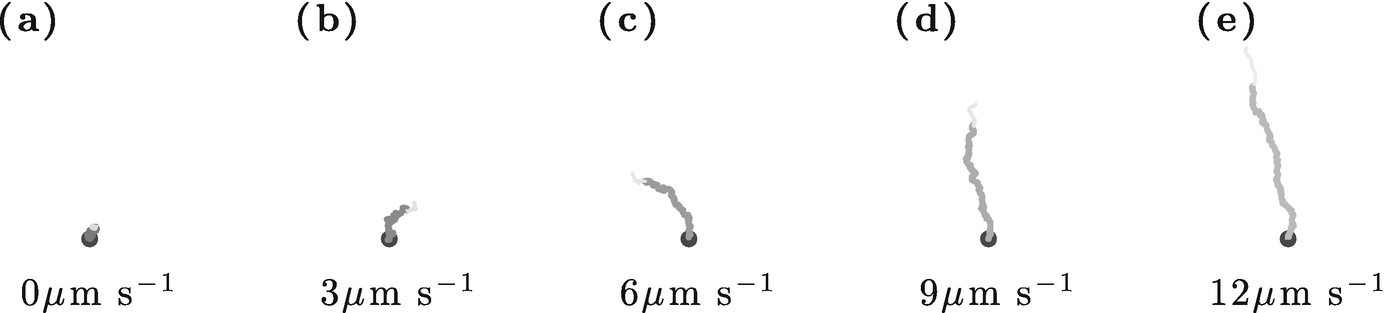
\includegraphics[width=1.0\linewidth]{462743_1_En_7_Fig2_HTML.png}
\caption{From passive to active Brownian motion. Displacement (gray path) from (a) Passive Brownian motion and (b–e) active Brownian motion for increasing self-propulsion speeds for a constant amount of time \cite{Toschi}}
\label{fig:displacement}
\end{figure}

Due to exhibiting movement mostly from thermal noise, passive Brownian particles exhibit purely diffusive motion.  Upon the addition of self-propulsion, the active force dominates over the thermal noise, enabling ballistic motion at short and diffusive at long time scales relative to the rotational diffusion rate, the slopes of which depend on the distance traveled before randomly reorienting, or the persistence length \cite{Toschi}.  Eqn.~\ref{Pe} is merely a non-dimensional form of the persistence length ($l_{\text{p}}$) that accounts for particle species of varying sizes:

\begin{equation}\label{area}
    l_{\text{p}} = v_{\text{p}} \tau_{\text{r}}
\end{equation}

\begin{figure}[ht]
\centering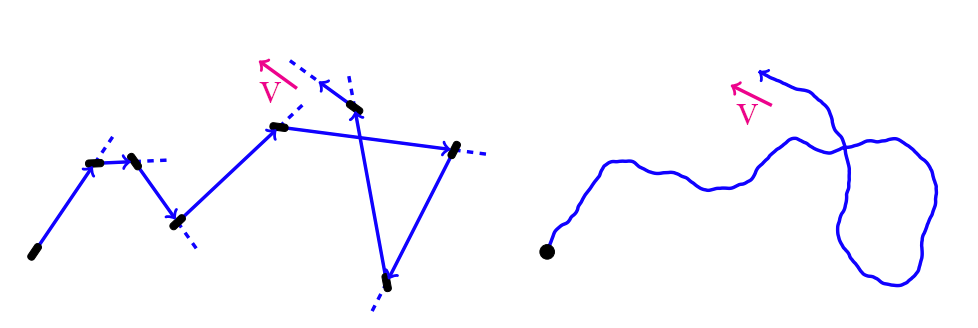
\includegraphics[width=0.9\linewidth]{Screen Shot 2020-08-12 at 8.07.17 AM2.png}
\caption{Simulated paths of a run-and-tumble (Left) and an active Brownian (Right) particles at short time scales (5 RTP re-orientations).  Each is diffusive at large length and time scales. \cite{Cates6}}
\label{fig:motion}
\end{figure}

Though comparable to run-and-tumble particles (RTPs), active Brownian particles (ABPs) notably differ in their rotation mechanism. ABPs experience constant rotational diffusion that is thermal in nature, allowing only for small angular variations at each time step unlike the potentially large angular variations seen in RTPs.  The difference in motion at short time and length scales can be seen in Figure \ref{fig:motion}.  When longer length and time scales are considered, there is a leading-order exact equivalence between ABPs and RTPs so long as the motility is independent of orientation \cite{Tailleur}.  

\section{Monodisperse Active System}\label{monodisperseABPactivity}

Foreign to purely passive Brownian systems, ABPs are experimentally \cite{Palacci, Theurkauff} and theoretically \cite{Redner, Bialke, Stenhammar4} found to enter a unique and dynamic metastable clustering state [Figure \ref{fig:three graphs}a] \cite{Speck}.  This motility-induced phase separation (MIPS) occurs via spinodal decomposition [Figure \ref{fig:three graphs}b] into a dynamic, nonequilibrium cluster, the high-density liquid phase, and a dilute, low-density gas phase \cite{Stenhammar3}.  Phase separation is found to be the result of a density dependent velocity, $v(\rho)$.  MIPS is similarly seen in RTP systems due to $v(\rho)$ \cite{Cates}, upholding the ABP-RTP equivalence under MIPS.


\begin{figure}[ht]
     \centering
     \begin{subfigure}[b]{0.5\textwidth}
         \centering
         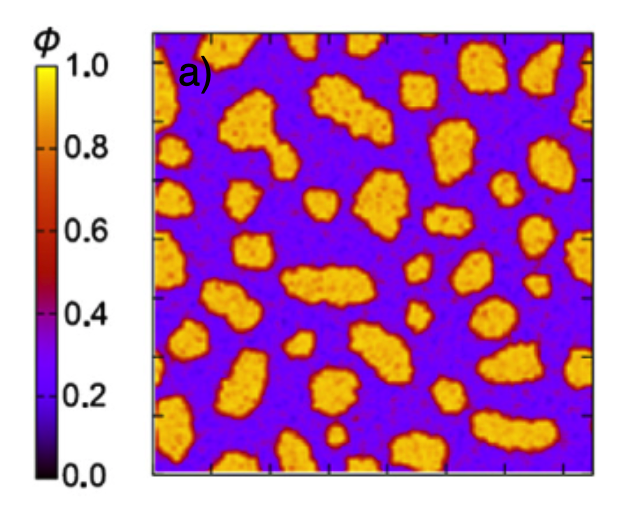
\includegraphics[width=\textwidth]{Screen Shot 2020-08-12 at 9.24.03 AM (1).png}
         \label{fig:mips}
     \end{subfigure}
     \hfill
     \begin{subfigure}[b]{0.45\textwidth}
         \centering
         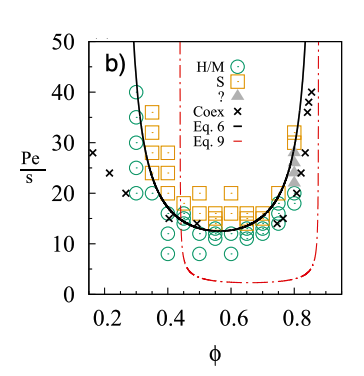
\includegraphics[width=\textwidth]{Screen Shot 2020-08-12 at 11.49.03 AM.png}
         \label{fig:phase2}
     \end{subfigure}
        \caption{a) ABP system in 2D undergoing MIPS color-coded by the local packing fraction, $\phi=\rho/\rho_0$.  Significantly higher density is seen in the clustered, dense phases (orange-yellow) than the gas phase (purple-blue) \cite{Gonnella}. b) Stability phase diagram for ABPs. Circles, squares, and triangles correspond to no phase separation, phase separation, and undetermined phase separation respectively An 'X' marks the coexisting volume fractions. The full lines correspond to the theoretical prediction for the spinodal line \cite{Nie}.}
        \label{fig:three graphs}
\end{figure}

As the local density increases, so does the rate of collisions, reducing the average effective particle velocity in that region \cite{Tailleur, Cates}.  Velocity decreasing with greater density results in small, metastable clusters that either immediately break apart and disperse into the gas phase or act as a nucleation site for cluster growth. As more particles move into this low-$v(p)$ region, they can collide with and be adsorbed by the nucleation site, becoming an edge particle that spatially confines the interior particles while still allowing freedom to rotate. These exterior edge particles are maintained so long as their orientation remains below the surface curvature horizon, i.e. $\hat{n}\cdot\hat{v}$ where $\hat{n}$ is normal to the surface \cite{Cates}. 

Upon relating the particle fraction of each phase to the ABP activity, a binodal envelope is established that is solely a function of activity \cite{Redner}.  At a certain critical activity, the system begins to phase separate and continues to do so to an increasing extent as the system becomes more active.  This binodal contradicts prior expectations that greater activity will destabilize the system, meaning effective temperature is not an effective description of activity as initially thought \cite{Schwarz-Linek}.  Because the binodal envelope is athermal in nature, this phase diagram is thus analagous to that of an equilibrium system of mutually attracting particles \cite{Nguemaha}, with Pe acting as an attraction strength. 

Though this may not make sense in terms of temperature, one can look at it in terms of kinetics. The growth and steady-state of the cluster can be thought of in terms of rates of adsorption to and desorption from the cluster, which are both activity dependent. While the rate of adsorption is greater than desorption, the cluster grows, and as soon as the rates become equal, the system has entered steady-state.  In other words, While the collision rate is greater than the rotational diffusion constant, the cluster grows.  Upon the two rates equating, the system enters stead-state, maintaining a dynamic cluster of approximately constant size \cite{Redner}. The mechanism of phase separation in monodisperse active systems is central to this thesis because it still holds for active mixtures despite the added complexities of a second activity.

\section{Active/Passive Mixtures}\label{activepassiveABPactivity}

Active/Passive mixtures introduce a second component into the equation which complicates the system significantly.  Similarly, there is now a scale of active:passive concentrations and, in turn, whole new phenomena introduced for each regime.  Systems can be predominantly passive with relatively few active particles, comparable concentrations of active and passive concentration, and predominantly active with relatively few passive particles.  

Ni et al.\cite{Ni,Ni2} demonstrated with numerical simulations that the glassy transition and kinetic arrest of highly supersaturated solutions can be overcome by doping the system with a small fraction of active particles, as little as $1\%$  of the system size.  

\begin{figure}[ht]
\centering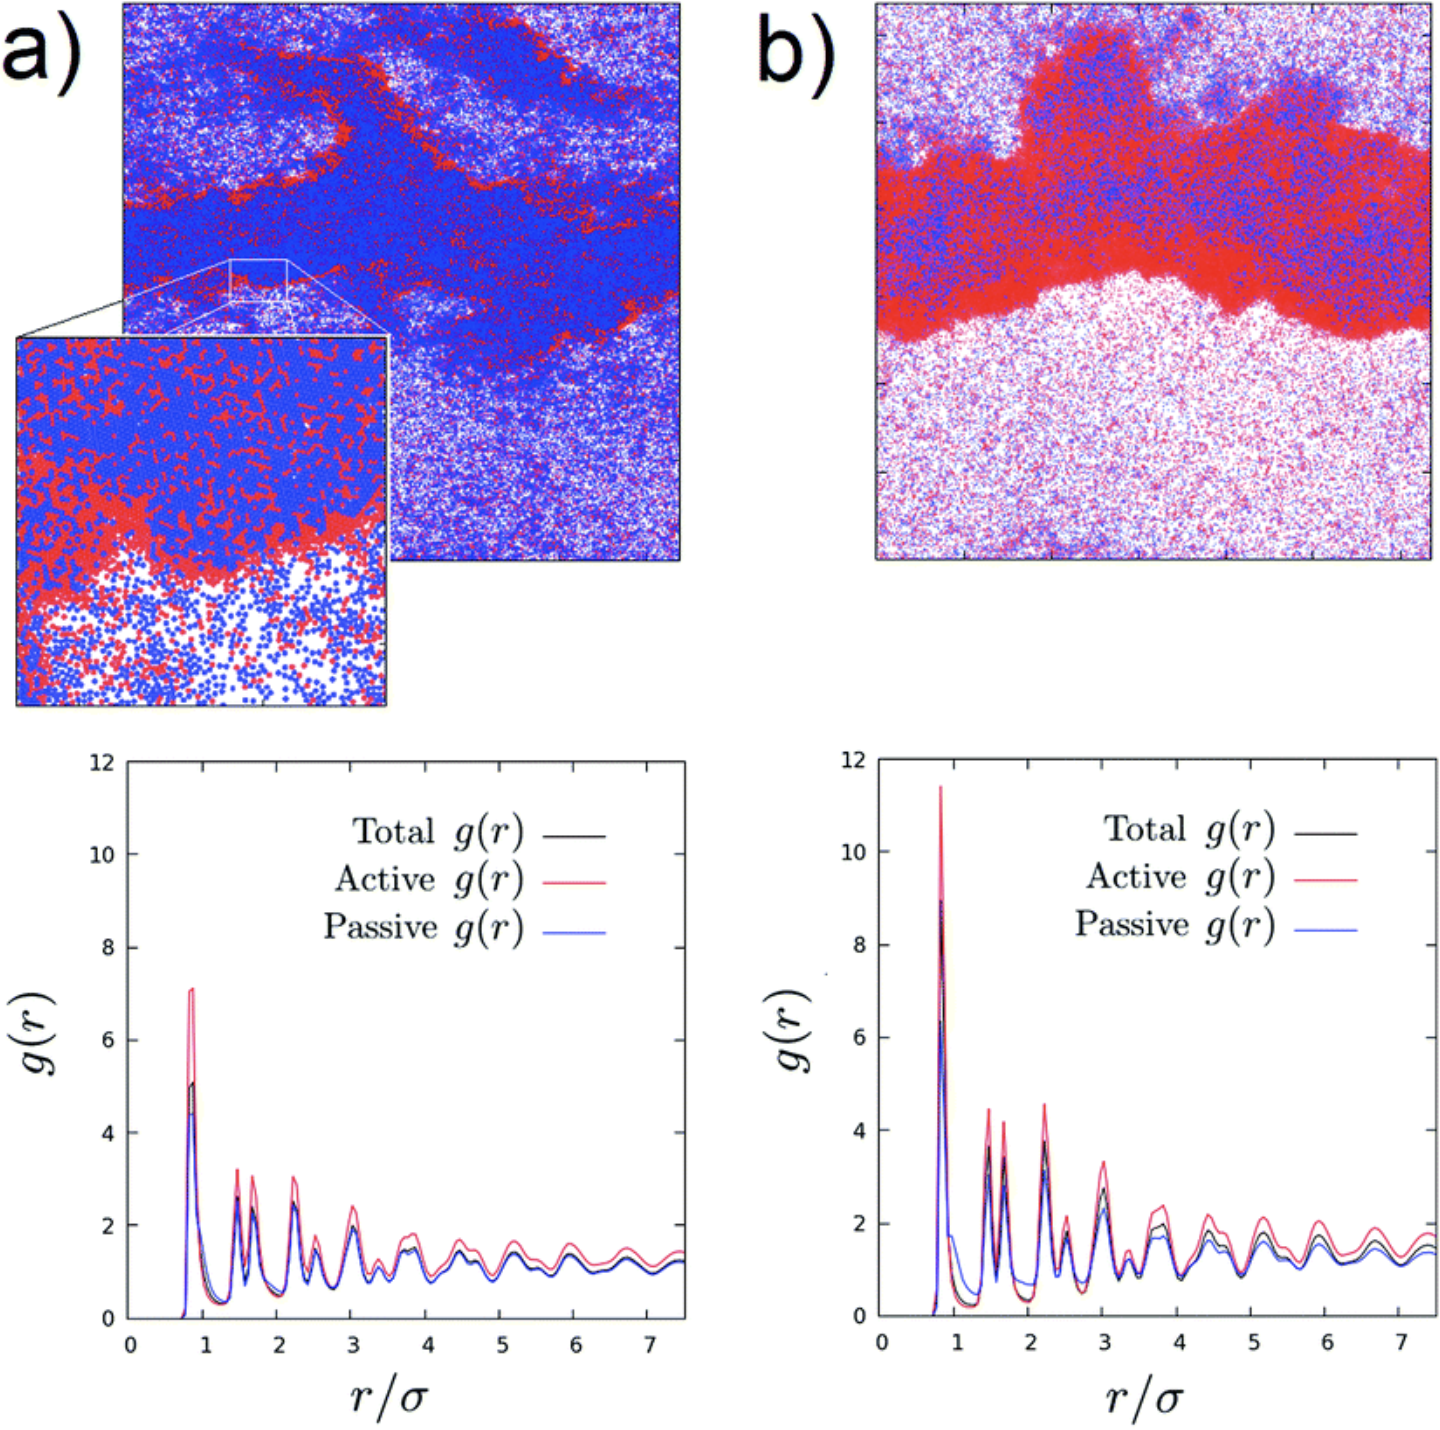
\includegraphics[width=0.8\linewidth]{Screen Shot 2020-08-10 at 9.55.19 AM.png}
\caption{Top: Snapshots of phase-separated mixtures of
passive (blue)/active (red) colloids: (a) $\phi_\text{p}$ = 0.6, Pe = 190,
(b) $\phi_\text{p}$ = 0.3, Pe = 170. Bottom: Radial distribution functions
corresponding to the top panels. \cite{Rodriguez} }
\label{fig:RDF}
\end{figure}

Kummel et al.\cite{Kummel} discovered that the degree of benefit or harm of the active particles is strongly dependent on the particle fraction of the active species.  At very low passive particle concentrations, above a minimum passive particle concentration, the active species begin to herd the passive particles into small, metastable clusters of passive particles surrounded by an active particle edge.  As the concentration of passive particles is further increased, activity-assisted crystallization becomes more effective and larger clusters are formed.  By looking at the radial distribution function (RDF), Rodriguez et al.\cite{Rodriguez} concluded that the the cluster structure is crystal-like at short distances and liquid-like at long distances [Figure \ref{fig:RDF}].  The active particle RDF is more well-defined than that for passive agents, suggesting that active agents force clustering of passive particles as if there were an effective attraction between them.  At the threshold of spontaneous crystallization, the active particles locally melt the surrounding lattice by self-propelling through the crystal domains, inducing defects in the region. The reduced resistance to active particle motion from defects results in the active particles concentrating at the domain interfaces, leading to permanent melting and recrystallization of these regions \cite{Kummel}.

Van Der Meer et al. \cite{Meer} utilized active dopants in simulations to transform polycrystalline material into a single crystal . Since active dopants are attracted to and generate defects, they are localized at grain boundaries.  As the concentration of these active particles were increased, so too were both their concentration at the grain boundaries and, in turn, grain boundary mobility, leading to significant coarsening of the domains over time [Figure \ref{fig:crystal}].  By turning off the activity, through means such as light-activated propulsion, the remaining defects crystallized, and the polycrystalline material became a single crystal.  

\begin{figure}[ht]
\centering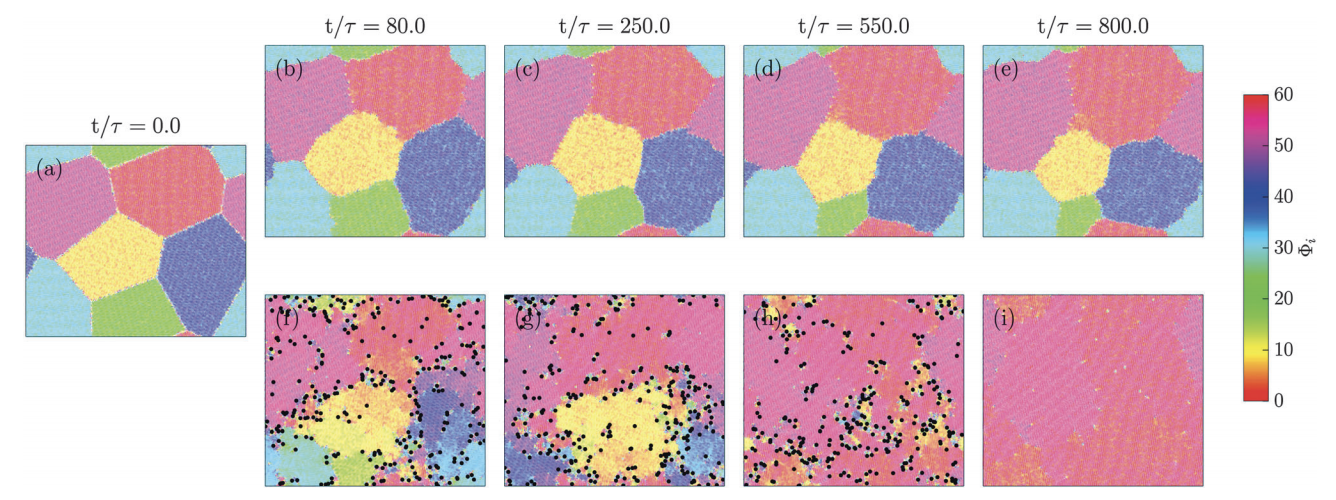
\includegraphics[width=1.0\linewidth]{Screen Shot 2020-08-12 at 12.21.43 PM.png}
\caption{Grain growth in a passive system (a–e) vs. a doped system (a and f–i). Color indicates the local orientation of a particle. Active particles are plotted in black. After the activity of the self-propelled particles is switched off, universal alignment proves the polycrystal has coarsened significantly in the active system compared to its passive counterpart. \cite{Meer} }
\label{fig:crystal}
\end{figure}

Mixtures of active/passive systems can also be used to promote transport within various confinements. Under purely Brownian motion, passive particles merely diffuse slowly through a channel.  Without use of an external field, Ghosh et al. \cite{Ghosh} demonstrated that by doping the passive Brownian system with a small fraction of ABPs, fast transport via a symmetry-directed particle flow through the channel is enabled by dragging passive particles along (autonomous pumping).

Stenhammar et al. \cite{Stenhammar2} investigated the influence of activity, active and passive particle fraction, and total particle packing fraction on the clustering of active/passive systems. When compared to their monodisperse counterparts, the dynamics of phase-separating mixtures is much more violent, with clusters constantly moving, fissioning, and merging.  This difference between active/passive and monodisperse active was further emphasized by Wittkowski et al. \cite{Wittkowski} who showed that spinodal instability can be associated with either a stationary bifurcation, also possible in monodisperse active systems, or a Hopf bifurcation.  The Hopf bifurcation is only possible in active/passive systems and results in moving clusters, explaining the newly seen dynamic nature for active/passive mixtures.

In addition to activity, the dependence of phase separation on total particle packing fraction and active particle packing fraction was established [Figure \ref{fig:binodal}]. Increasing the concentration of active particles, either through increasing the active particle fraction or total particle packing fraction, is found to result in a greater incidence of clustering at lower activities \cite{Stenhammar2}.  

\begin{figure}[ht]
\centering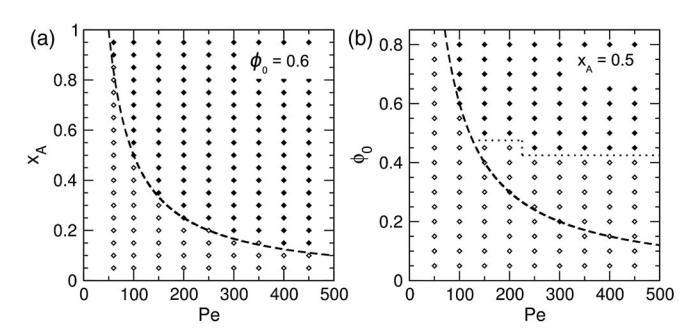
\includegraphics[width=0.9\linewidth]{Screen Shot 2020-08-10 at 9.39.25 AM.png}
\caption{a) Phase diagram in the $Pe-X_\text{A}$ plane in 2D for $\phi_0=0.6$. b) Phase diagram in the $Pe-\phi_0$ plane for $X_\text{A}=0.5$.  Black-filled points represent phase separation occurring and white-filled points represent a homogeneous system. \cite{Stenhammar2} }
\label{fig:binodal}
\end{figure}

\section{Active/Active Mixtures}\label{activeactiveABPactivity}

Activities have been treated as a scalable continuum that can determine phase separation, yet we maintained the passive species at a constant zero activity.  This corresponds to a single case in an active/active mixture where one activity is held at a constant $Pe=0$, raising the question of what would happen if both activities were allowed to vary.  

Activity can be controlled in two ways: system temperature \cite{Stenhammar3, Stenhammar2, Wittkowski} or preferred swim speed \cite{Kolb}. To see the effect of this, we can re-write eqn. ~\ref{2} to be dimensionless as \cite{Preisler}:

\begin{equation}\label{74}
    0=\frac{D_\text{t}}{k_\text{B}T}\left[\boldsymbol{F}_{\text{C}}+\boldsymbol{F}_{\text{D}}+\boldsymbol{F}_{\text{A}}+\boldsymbol{F}_{\text{S}}\right]
\end{equation}

\noindent where $D_\text{t}=k_\text{B}T/\gamma$.  This simplifies to:

\begin{equation}\label{75}
        \dot{\boldsymbol{r}_{\text{i}}} =\frac{D_\text{t}}{k_\text{B}T} \boldsymbol{F}_{\text{C}}(\boldsymbol{r}_{\text{i,j}})+v_0\boldsymbol{\hat{p}_{\text{i}}}+\sqrt{2D_\text{t}}\boldsymbol{\Lambda}^{\text{t}}_{\text{i}}
\end{equation}

\noindent Defining the temperature of our system of active Brownian particles by a dimensionless effective temperature ($T^\prime = k_\text{B}T/\epsilon$) where the interaction strength in the WCA potential, $\epsilon$, is varied to change the effective temperature:

\begin{equation}\label{76}
        \dot{\boldsymbol{r}_{\text{i}}} =\frac{D_\text{t}}{\epsilon T^\prime} \boldsymbol{F}_{\text{C}}(\boldsymbol{r}_{\text{i,j}})+v_0\boldsymbol{\hat{p}_{\text{i}}}+\sqrt{2D_\text{t}}\boldsymbol{\Lambda}^{\text{t}}_{\text{i}}
\end{equation}

\begin{equation}\label{phi3}
    \dot{\theta}_{\text{i}} = \sqrt{2D_\text{r}}\Lambda^r_\text{i}
\end{equation}

By utilizing eqn. ~\ref{LJForce} and identifying that $D_\text{t}=\epsilon T^\prime/\gamma$, we see that varying the effective temperature ($T^\prime$) via the interaction strength ($\epsilon$) will only change the magnitudes of rotation and the Brownian component of translation ($\boldsymbol{F}_\text{S}$).  As system temperature (T) increases via increasing $\epsilon$, the translational and rotational diffusion constants also increase.  The increase in translational diffusion is still negligible compared to the active force in eqn.~\ref{2}, but thermal diffusion is the only determinant of rotation rate in eqn.~\ref{3}.  As a result, increasing the system temperature will decrease the reorientation time and, in turn, the time that particles travel in a single direction, resulting in decreased activity per eqn ~\ref{Pe}.  This is different from the velocity-variant model where preferred swim speed is instead varied to alter the activity.  

Though both models agree for active/passive mixtures \cite{Stenhammar2}, the benefits of the velocity-variant model become evident upon looking at active/active mixtures.  When a system enters a dynamic clustered state, the growth, size, and stability of the cluster is determined by the rates of adsorption and desorption of particles at the edges \cite{Redner, Redner2}.  In the temperature-variant model of a binary active mixture, the slow species, with increased reorientation rate, is more likely to escape from the cluster edge than the fast species, resulting in a predominantly fast edge.  Biasing the desorption rate will, in turn, bias the cluster formation and composition.

\begin{figure}[ht]
\centering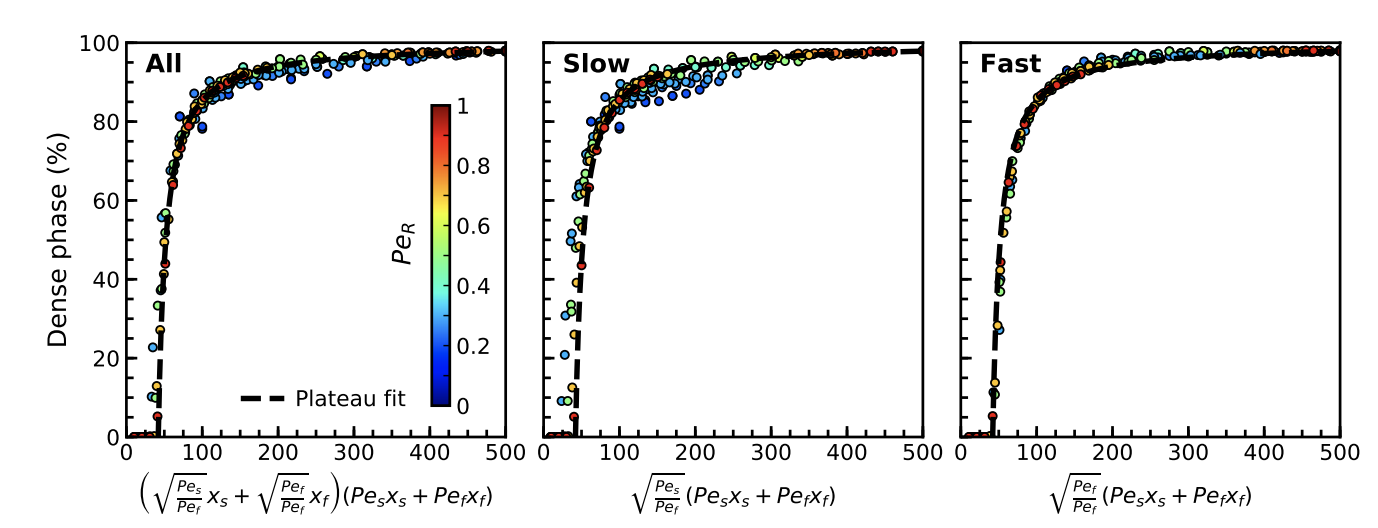
\includegraphics[width=1.0\linewidth]{Screen Shot 2020-08-10 at 12.35.19 PM.png}
\caption{Steady-state percentage of particles in the dense phase plotted against net activity weighted by different activity-ratios. The data collapses onto a plateau function (ax/b + x) where a = 100 (maximum percent in the dense phase) and b = 10. \cite{Kolb}}
\label{fig:netpe}
\end{figure}

Kolb et al. \cite{Kolb} searched for an underlying factor that determines phase separation in a binary active/active mixture of fast and slow hard spheres. There were two activity-pairing regimes:  Regime I corresponded to active/passive and active/weakly-active systems and regime II is active/active systems.  Regime I demonstrated large segregation in the cluster by particle type with a predominantly fast edge and domains of slow particles populating the interior.  Slow particles were enhanced while fast particles were suppressed from entering the dense phase compared to either a monodisperse slow or fast system respectively.  These effects decayed asymptotically until becoming an active/active system (Regime II), the dense phase was homogeneously mixed and each species participated as it would in its respective monodisperse system.  Phase separation was found to have a strong dependence on net activity [Figure \ref{fig:netpe}] given by:

\begin{equation}\label{netpe}
    Pe_\text{net}=(x_\text{s}Pe_\text{s}+x_\text{f}Pe_\text{f})
\end{equation}

\subsection{Course-grained Theories}

In a passive system, hot and cold particles would equilibrate to a single temperature.  In an active system, when particles collide, the particles slow down but then accelerate back to their preferred swim speed.  This raises the question: is there a value that equilibrates in an active matter system?  The swim temperature definition, $T_\text{s}=\zeta U_0^2 \tau_\text{R}/(6k_\text{s})$, is an intrinsic kinetic temperature that is not shared between particles and, therefore, does not equilibrate, begging the question of what does equilibrate \cite{Takatori}.

Takatori, et al. \cite{Takatori} and Yang, et al. \cite{Yang2} developed a notion of a mechanical swim pressure that arises from the particle's active force acting on the confinement boundary, which is entirely athermal in nature.  Utilizing an approximate generalized free energy of the system, Takatori's swim pressure can be utilized to form a qualitative phase diagram that can predict phase separation in active/active mixtures [Figure \ref{fig:two graphs}a] \cite{Takatori2}. When increasing the area fraction of the system, the swim pressure decreases, pushing the system towards phase separation. On the other hand, increasing area fraction also increases the interparticle pressure monotonically, deterring phase separation. The competition between these two effects is determined by the reorientation P\'{e}clet number, $Pe_\text{R}=\frac{a}{(U_\text{0}\tau_\text{r})}$ [Figure \ref{fig:two graphs}b] \cite{Takatori3}.

\begin{figure}[ht]
     \centering
     \begin{subfigure}[b]{0.5\textwidth}
         \centering
         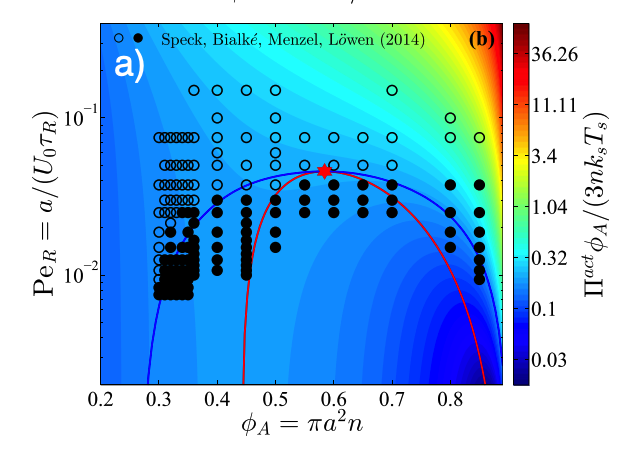
\includegraphics[width=\textwidth]{Screen Shot 2020-08-07 at 10.53.40 AM.png}
         \label{fig:pressure}
     \end{subfigure}
     \hfill
     \begin{subfigure}[b]{0.45\textwidth}
         \centering
         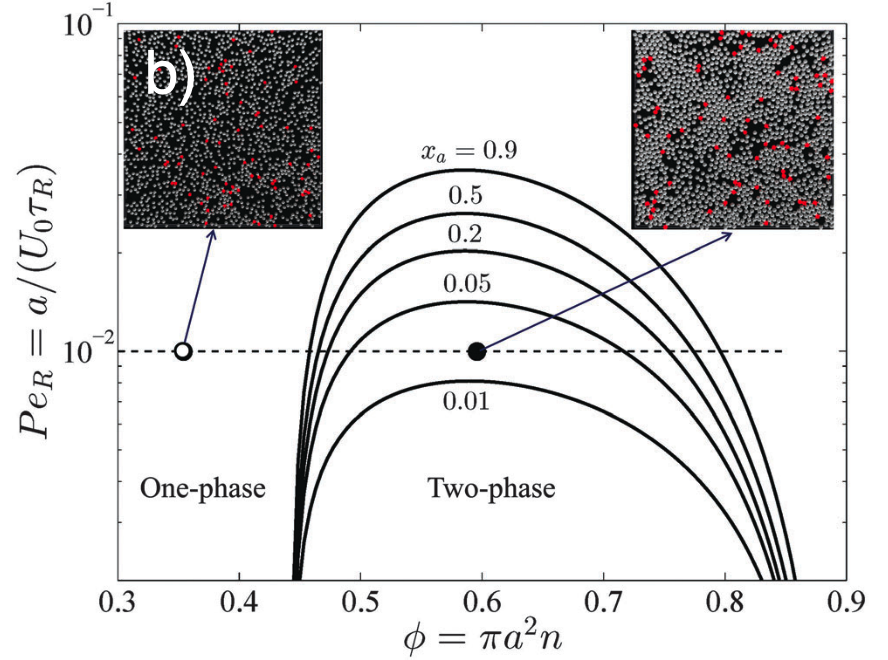
\includegraphics[width=\textwidth]{Screen Shot 2020-08-13 at 1.57.21 PM.png}
         \label{fig:densbin}
     \end{subfigure}
        \caption{a) Phase diagram in the $Pe_\text{R}-\phi$ plane in 2D. The color bar shows the active pressure scaled with the swim energy. The blue and red curves are the binodal and spinodal, respectively. The critical point is shown with a red star. The open and filled symbols are simulation data for a homogeneous and phase-separated state respectively. \cite{Takatori2}. b) Phase diagram in the $Pe_\text{R}-\phi$ plane in 2D for different $X_\text{a}$. The solid curves are the spinodals. The two-phase region diminishes as $X_\text{a}$ decreases. Two steady state images from simulation are shown. The red and white circles are the active and passive particles, respectively \cite{Takatori3}.}
        \label{fig:two graphs}
\end{figure}

Solon et al. \cite{Solon2} instead built a generalized theory of phase-separating active matter, applicable to both quorum-sensing and pairwise-force active particles, starting from a generalized Cahn-Hilliard hydrodynamic description.  Solon's approach requires information of both the bulk phase and bulk-gas interface in order to get their predictions of the binodal. Hermann et al. \cite{Hermann} developed a microscopic theory for bulk and interfacial behavior of ABPs by utilizing power functional theory \cite{Schmidt}.  Separating the one-body force density into four components (isotropic drag, interfacial drag forces against the forward motion, superadiabatic spherical pressure gradient, and the quiet life gradient force), an equilibrium pressure and chemical potential is found to explain nonequilibrium phase coexistence.  The balance of the quiet life force and the opposing adiabatic forces, both of which are independent of interfacial contributions, is found to determine bulk coexistence.  The total chemical potential profile is found to arise from the sum of ideal, adiabatic excess, and quiet life contributions.

Van Der Meer et al. \cite{Van} expanded upon this by using mechanical pressure as a starting point to look into the mere existence of a chemical equilibrium between the dense and gas phases.  In classical statistical physics, a chemical potential arises when the system is connected to a particle reservoir.  The chemical potential is directly related to the density of the reservoir.  This idea was imitated in simulation where an active/active mixture was connected to a monodisperse active reservoir by a semipermeable membrane that only allows the initially reservoir's activity species to pass through.  Over time, a steady state reservoir density is reached, confirming the existence of a chemical potential.  They further found that the gas-liquid coexistence for an active/active mixture can be fully described by the local normal pressure and the reservoir density.  The two, theoretical binodals predicted by pressure and reservoir density collapse into a single binodal, which is in good agreement with simulation data.


\section{Other Mixtures}
\subsection{Mixtures of Activity Mechanism(s)}\label{propulsionmech}
Though mixtures of different activities are possible, so too are different forms of active matter.  Khatami et al. \cite{Khatami} demonstrated that through the use of a circular, Matryoshka-like maze obstacles with nested shells, mixtures of ABPs and RTPs are able to be filtered out and differentiated. ABPs are capable of escaping from the center faster whereas RTPs can reach the center from the rim more easily. Due to its small orientation fluctuations and the convex boundaries, the mean ABP orientation fluctuates around the surface normal, resulting in the particle sliding along the boundaries via short drift motions that resemble a random walk \cite{Fily}. The RTP constantly tumbles and detaches from the wall.  Upon arriving at an opening from the outside of the maze, entering the opening relies on the ability for a particle to reverse direction and head towards the inner parts of the maze, which is much more likely for a tumble event.


\begin{figure}[ht]
\centering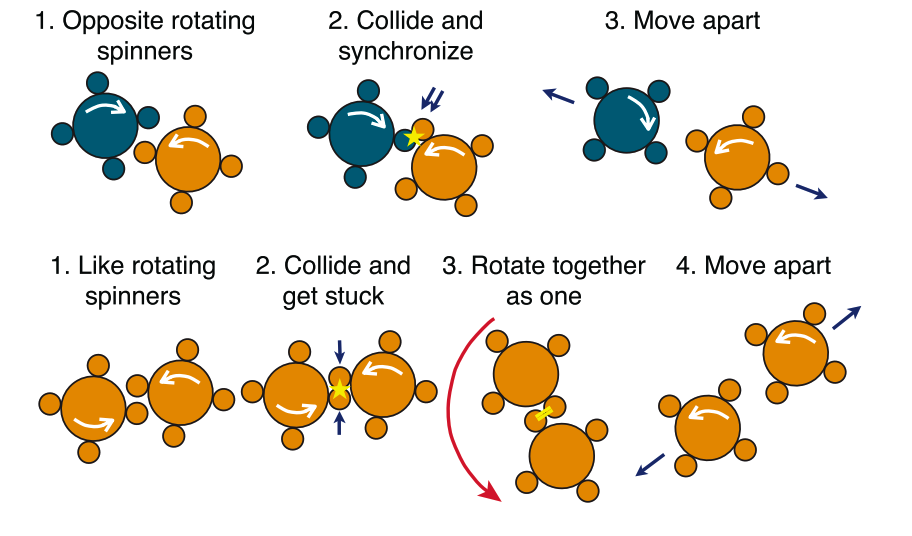
\includegraphics[width=0.9\linewidth]{Screen Shot 2020-08-14 at 2.32.32 PM.png}
\caption{Interaction mechanism of a) two opposite chirality spinners and b) two same chirality spinners \cite{Nguyen}}
\label{fig:collide}
\end{figure}

Not only can particles actively translate through space but also rotate.  Nguyen et al. \cite{Nguyen} considered mixtures of chiral (clockwise and counter-clockwise rotating) spinners.  Macroscopic spinners submerged in a fluid \cite{Grzybowski, Grzybowski2} can experience hydrodynamic interactions \cite{Drescher, Ischikawa} that are either repulsive or attractive in nature due to the formation of vortices \cite{Han, Kokot}. At low densities, the system is in a frozen, constantly rotating state \cite{Hinrichsen}.  At higher densities, the time interval between collisions decreases to such a point that non-stop chained collisions [Figure \ref{fig:collide}] can maintain the transfer of rotational to translational motion \cite{Nguyen}.  Yeo et al. \cite{Kyongmin} added passive particles to this density regime.  Instead of spinners of like-chirality pairing, opposite-chirality pairing was more likely due to the long-range fluid flow from the spinner-induced motion of passive particles.  Scholtz et al. \cite{Scholz} demonstrated phase separation by spinodal decomposition in oppositely rotating robots.  At very high densities, the colloidal spinner system crystallizes \cite{Nguyen}. The spinners synchronize and rotate collectively around the crystals center of mass instead of their own center of mass, making an active, rotating crystal.  As the activity of the spinners increases, the density at which crystallization occurs decreases \cite{Redner, Bialke2}.  

Increased complexity can be added to an active spinner system by introducing a swim velocity, inducing chiral circular motion similar to bacteria near a surface \cite{Lemelle}.  Reichhardt et al. \cite{Reichhardt} utilized an asymmetric array to separate the active molecules in terms of both chirality and swim radius based upon the number of interactions with the substrate.  Chen et al. \cite{Chen5} expanded upon Reichhardt's work by employing two oppositely rotating obstacles to sort circularly moving mixtures based on chirality.  Ai et al. \cite{Ai} further delved into mixing/demixing of active systems by adding local velocity alignment interactions, in the manner of Vicsek \cite{Vicsek}, to the particles.  When the chirality difference competes with the polar velocity alignment, particles aggregate into two separate clusters dependent on their direction of rotation.

\subsection{Role of Non-Steric Interparticle Forces}\label{interactionmech}

When colloidal particles are composed of or coated with magnetic materials, such as magnetic Janus particles \cite{Ren}, they become responsive to external fields and show unique, dynamic behavior experimentally, such as circular motion of an active magnetic particle in a rotating magnetic field \cite{Cebers}, clustering of magnetotactic bacteria in an external magnetic field \cite{Rupprecht, Meng}, and many others \cite{Chen, Erb, Snezhko, Snezhko2}.  

Yang et al. \cite{Yang3} demonstrated the ability for an active/passive mixture to phase and flow separate using paramagnetic swimmers in a channel. The system consists of a binary mixture of passive particles with different charges and sizes. These particles interact through repulsive dipole-dipole potential, $V_\text{i,j}=Q_\text{i}Q_\text{j}/|r_\text{i}-r_\text{j}|^3$ where $Q_\text{i/j}$ is the effective charge.  A small concentration of light-driven, paramagnetic micro-swimmers (MS) separates the flow of the system into four regimes dependent on the activity: rigid body motion, inverse velocity motion, strong flow separation, and fast MS motion. As the activity is increased, the MS can locally melt the material (inverse velocity motion), breaking the system out of solid state (rigid body motion). In the strong flow regime, the system phase separates due to greater friction, enabling small particles to move faster than large particles. 

Phase separation of dipolar systems can result in a variety of structures, such as ordered phases including face-centered-cubic, hexagonal-close-packed, and body-centered-tetragonal at high packing fractions, and fluid, string-fluid, and gel phases at low packing fractions \cite{Goyal, Schmidle, Halsey}.  Maloney et al. \cite{Maloney} expanded upon the previously passive systems by adding ABPs to the system.  Slow-moving ABPs are found to enhance clustering compared to their passive counterparts while maintaining similar structure to that prior to the addition of ABPs.  As the activity is increased, the active particles can break apart the dipolar chains and MIPS is observed.

\subsection{Role of Particle Softness}\label{softnessmix}

While the importance of rigid particle structures in a colloidal system is clear, soft particle systems have not yet been discussed.  Many species utilize shape deformation in their locomotion in both biology, such as microorganisms in the very low Reynolds number regime \cite{Trouilloud} and cells \cite{Killich, Maeda}, and inorganic colloidal systems, like self-propelled oil droplets in an oil-water mixture \cite{Sumino}.   Softness can arise in one of two ways: either the interaction potential allowing for some degree of compression beyond the particle radius, i.e. the scaling of $\epsilon$ in eqn. \ref{LJ} \cite{Levis}, or the particles themselves which can be elastic and deformable, i.e. microgels and emulsions.  The particle softness can induce large changes system properties \cite{Seekell, Nigro, Mattsson, Nicoletta}. 

\begin{figure}[ht]
\centering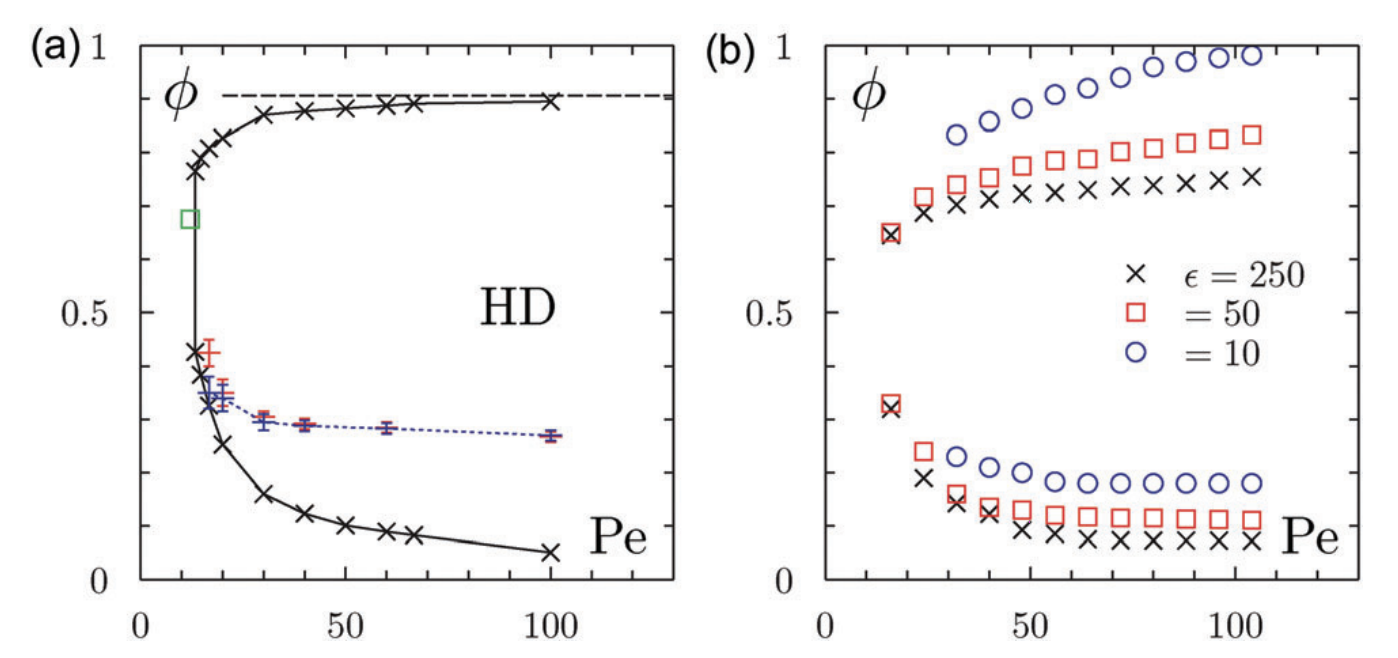
\includegraphics[width=1.0\linewidth]{Screen Shot 2020-08-11 at 10.06.26 PM.png}
\caption{$Pe-\phi$ phase diagram of ABP. Left: Active Brownian-Hard Disks (infinite hardness). Black symbols show the coexisting densities defining the binodals. Red points indicate the onset of MIPS. Blue points correspond to the location of the pressure drop. Right: ABPs of different softness.  \cite{Levis}.}
\label{fig:softness}
\end{figure}

Levis et al. \cite{Levis} found that increasing particle softness shifted the density of the liquid phase to higher values, and increased the activity at which phase separation occurs [Figure \ref{fig:softness}].  Utilizing the surface tension derived by Omar et al \cite{Omar3}, Kolb et al \cite{Kolb2} found that despite different particle softness as defined by the WCA potential, the equilibrium surface tension of the liquid phase remained constant at constant activity for a monodisperse system. Kolb et al \cite{Kolb} further delved into soft mixtures looking at binary active mixtures of varying softnesses.  Similar to hard sphere mixtures, soft sphere mixtures exhibit a binodal which depends on net activity.  More interestingly, the possibility of phase re-entrance with activity is demonstrated, which calls into question the interpretation of activity as an attraction between colloids \cite{Redner2}. In addition, the composition of the dense phase changes to a predominantly fast interior and slow edge in soft sphere mixtures \cite{Kolb2} as opposed to a predominantly slow interior and fast edge as seen in hard spheres \cite{Kolb}.





\subsection{Mixtures of Shapes and Sizes}\label{shapessizes}

Few systems in real life, especially biological systems, are perfectly homogeneous in terms of both shape and size.  There is a wide array of diversity present in active systems, such as the interior of a cell, that can have any number of influences on the active species capabilities.  

In a mixture of micromolecules suspended in a solution of macromolecules, an attractive depletion force can arise between macromolecules due to an unbalanced osmotic pressure exerted on them by the surrounding micromolecules \cite{Asakura}.  As dissimilarity between particle size is increased, so too is the influence of this interaction, leading to aggregation of particles of both sizes \cite{Asakura2}.  For size ratios (large:small particle size) particles greater than five, purely entropy-driven clustering of the system occurs \cite{Biben, Frenkel}.  Wu et al. 

Dolai et al. \cite{Dolai} expanded this to ABPs by looking at a system of soft, spherical particles consisting of both large, passive and small, active particles.  As either the size ratio or active particle fractions increases, the system begins to phase separate more due to the depletion force. The depletion force between active and passive species can be either attractive or repulsive depending on the effective velocity of passive particles.  As both the size ratio of passive:active particles and the active particle fraction increases, the number of collisions of active with passive particles increases, resulting in a greater effective velocity for passive particles.  As passive particles become faster, they are no longer regions of low motility and do not seed MIPS.  In this case, passive particles have both an effective repulsion towards active particles and an effective attraction towards other passive particles, resulting in a phase separation into large, HCP clusters. 

\section{Conclusion}

Currently, the field focuses on monodisperse single-component active systems. However, both in nature and in materials design, there is heterogeneity and many components. Though the complexity of these mixed, active systems is great, allowing for active mixtures opens an enormous parameter space and thus a host of opportunities in materials science.  These mixed systems display the same uniqueness of MIPS and non-equilibrium clustering as their monodisperse counterparts while adding even more diverse capabilities like activity induced transport \cite{Ghosh}, sorting \cite{Chen5}, enhanced crystallization \cite{Meer}, reduced degree of sedimentation \cite{Palacci4}, and even more unique and enhanced phase separation behavior \cite{Kolb}.  The aforementioned capabilities could serve to enhance many pre-existing technologies, such as increased crystallinity in optoelectronic devices \cite{Meer, Castro}, reduced sedimentation rate in cements \cite{Palacci4}, or superior performing robotic swarms for industrial applications \cite{Brambilla}.  Though its practical application in a variety of fields may be far off, characterizing and understanding these complicated, mixed systems is the next big step in bringing this promising concept to the forefront of human technology and innovation.

My project will contribute fundamental knowledge to the statistical mechanics and phase behavior of multi-component active matter (MCAM) through computationally intensive research. Natural mixtures are incredibly inhomogeneous, obscuring the influence of their many variables that dictate the system’s phase behavior.  In order to extend theoretical knowledge of the monodisperse system to that of real-life, inhomogeneous active mixtures must be studied systematically. To achieve this, I will 1) study the effect of varying activity, stiffness, size and concentration of each species on the phase behavior. I will then 2) study the same systems subject to various confinements. Finally, I will 3) utilize understanding from (1) and (2) to design the parameters of the mixture to obtain emergent behavior that does a specific useful task, specifically cancer-targeting drug delivery systems.

With increasing activity and system density, particles become increasingly more likely to collide, leading to a lower effective swim speed at increasing local densities and, in turn, MIPS in both monodisperse \cite{Theurkauff} and binary activity systems \cite{Kolb}.  My preliminary data shows that both particle activity and softness strongly influence the onset and degree of MIPS due to varying bulk pressure and, in turn, surface tension that maintains the liquid phase \cite{Kolb3, Lauersdorf}. As a result, I expect that other variables that influence the rate and strength of interaction will influence MIPS as well, but the question is how. Using Molecular Dynamics software [HOOMD-blue \cite{Anderson5}], I will perform Brownian Dynamics simulations to search for and study emergent behavior, such as phase transitions and stability in unconfined MCAM consisting of different combinations and concentrations of spherical active particles with variable driving forces, e.g. fast and slow, softness, and sizes. One important question I am addressing here is whether and under what conditions I can have MCAM phase separate into domains of the different components, like an active brazil-nut effect.

Many biological and synthetic active systems are finite and in confinement, such as within a vesicle or membrane. With the aim to discover ways to exploit confinement in order to induce and control the behavior of the system, I will also confine mixtures in different rigid and flexible geometries, as well as, flat and curved surfaces and will compare with findings in bulk. I expect interesting results because active rotator mixtures in confinement (coined “active colloidal cells” \cite{Van Anders, Nguyen} have shown a wealth of emergent behavior that was distinct from the unconfined case. My hypothesis is that the relative length-scales between the confinement and the extent of the dense phase will determine phase behavior and stability. Specifically, as confinement gets more comparable in size to the dense phase, I expect boundaries to frustrate phase behavior leading to novel steady states, bistability, and non-equilibrium phase transitions -- all of which will also depend on how rigid/flexible the boundary is.  Fixed shape and curvature of rigid boundaries can frustrate the assembly affecting the interior phase behavior. Flexible boundaries, on the other hand, will respond to active forces by changing their shape and curvature, which will also affect the phase behavior inside the boundary.

Building upon the previous two steps, I will apply our understanding of novel behaviors to perform useful tasks, such as the delivery of cancer-fighting drugs via active nanoparticles (NPs). My goal will be to inverse design the system’s emergent behaviors in order to form a homogeneous distribution of NPs around the tumor site. I will simulate MCAM of small active NPs that are weakly attracted to large cancer cells and confined under flexible boundary conditions to accurately represent the biological system. Self-propulsion has been shown to overcome the weakly attractive potential between agents and prevent aggregation \cite{Redner}. As a result, my system will have two modes: one where externally induced self-propulsion \cite{Palacci} prevents active NPs from sticking to tumor cells and another where the passive NP behavior is controlled by the attractive potential with the tumor cells.  My aim is to predict, tune, and define parameters for the active NPs, such as size, activity, softness, and the scalable attractive potential, under which the tasks are performed correctly and efficiently.  While also discovering and characterizing the collective behavior in active mixtures, my work aims to enable experimental study of self-propelling drug delivery agents by understanding the fundamental physics that dictate phase behavior. 


\newpage 
\begin{thebibliography}{9}

\bibitem{Schliwa}
Schliwa M, Woehlke G. Molecular Motors. Mol Mot. 2003;422:759-765. doi:10.1385/1597454907

\bibitem{Oriola}
Oriola, D. Julicher F., Brugues J. Active forces shape the metaphase spindle through a mechanical instability. PNAS. 2020;117(28):16154-16159. doi:10.4121/uuid

\bibitem{Drescher}
Drescher K, Leptos KC, Tuval I, Ishikawa T, Pedley TJ, Goldstein RE. Dancing volvox: Hydrodynamic bound states of swimming algae. Phys Rev Lett. 2009;102(16):1-4. doi:10.1103/PhysRevLett.102.168101

\bibitem{Zhang}
Zhang HP, Be’er A, Florin EL, Swinney HL. Collective motion and density fluctuations in bacterial colonies. Proc Natl Acad Sci U S A. 2010;107(31):13626-13630. doi:10.1073/pnas.1001651107

\bibitem{Peruani}
Peruani F, Starruß J, Jakovljevic V, Søgaard-Andersen L, Deutsch A, Bär M. Collective motion and nonequilibrium cluster formation in colonies of gliding bacteria. Phys Rev Lett. 2012;108(9):1-5. doi:10.1103/PhysRevLett.108.098102

\bibitem{Ballerini}
Ballerini M, Cabibbo N, Candelier R, et al. Interaction ruling animal collective behavior depends on topological rather than metric distance: Evidence from a field study. Proc Natl Acad Sci U S A. 2008;105(4):1232-1237. doi:10.1073/pnas.0711437105

\bibitem{Lopez}
Lopez U, Gautrais J, Couzin ID, Theraulaz G. From behavioural analyses to models of collective motion in fish schools. Interface Focus. 2012;2(6):693-707. doi:10.1098/rsfs.2012.0033

\bibitem{Mlot}
Mlot NJ, Tovey CA, Hu DL. Fire ants self-assemble into waterproof rafts to survive floods. Proc Natl Acad Sci U S A. 2011;108(19):7669-7673. doi:10.1073/pnas.1016658108

\bibitem{Hu}
Hu DL, Phonekeo S, Altshuler E, Brochard-Wyart F. Entangled active matter: From cells to ants. Eur Phys J Spec Top. 2016;225(4):629-649. doi:10.1140/epjst/e2015-50264-4

\bibitem{Zohdi}
Zohdi TI. Mechanistic modeling of swarms. Comput Methods Appl Mech Eng. 2009;198(21-26):2039-2051. doi:10.1016/j.cma.2008.12.029

\bibitem{Vicsek}
Vicsek T, Czirok A, Ben-Jacob E, Cohen I, Shochet O. Novel Type of Phase Transition in a System of Self-Driven Particles. Phys Rev Lett. 1995;75(6):1226-1229. doi:10.1016/0009-8981(74)90015-1

\bibitem{Romanczuk}
Romanczuk P, Erdmann U, Engel H, Schimansky-Geier L. Beyond the Keller-Segel model. Eur Phys J Spec Top. 2008;157(1):61-77. doi:10.1140/epjst/e2008-00631-1

\bibitem{Peruani2}
Peruani F, Deutsch A, Bär M. Nonequilibrium clustering of self-propelled rods. Phys Rev E - Stat Nonlinear, Soft Matter Phys. 2006;74(3):1-4. doi:10.1103/PhysRevE.74.030904

\bibitem{Wensink}
Wensink HH, Löwen H. Aggregation of self-propelled colloidal rods near confining walls. Phys Rev E - Stat Nonlinear, Soft Matter Phys. 2008;78(3):20-23. doi:10.1103/PhysRevE.78.031409

\bibitem{Yang7}
Yang Y, Marceau V, Gompper G. Swarm behavior of self-propelled rods and swimming flagella. Phys Rev E - Stat Nonlinear, Soft Matter Phys. 2010;82(3):1-13. doi:10.1103/PhysRevE.82.031904

\bibitem{Aranson}
Aranson IS, Volfson D, Tsimring LS. Swirling motion in a system of vibrated elongated particles. Phys Rev E - Stat Nonlinear, Soft Matter Phys. 2007;75(5):1-9. doi:10.1103/PhysRevE.75.051301

\bibitem{Drescher2}
Drescher K, Dunkel J, Cisneros LH, Ganguly S, Goldstein RE. Fluid dynamics and noise in bacterial cell-cell and cell-surface scattering. Proc Natl Acad Sci U S A. 2011;108(27):10940-10945. doi:10.1073/pnas.1019079108

\bibitem{Ghosh}
Ghosh PK, Misko VR, Marchesoni F, Nori F. Self-propelled janus particles in a ratchet: Numerical simulations. Phys Rev Lett. 2013;110(26):1-5. doi:10.1103/PhysRevLett.110.268301

\bibitem{Chen5}
Chen Q, Ai BQ. Sorting of chiral active particles driven by rotary obstacles. J Chem Phys. 2015;143(10). doi:10.1063/1.4930282

\bibitem{Meer}
Van Der Meer B, Filion L, Dijkstra M. Fabricating large two-dimensional single colloidal crystals by doping with active particles. Soft Matter. 2016;12(14):3406-3411. doi:10.1039/c6sm00031b

\bibitem{Palacci4}
Palacci J, Cottin-Bizonne C, Ybert C, Bocquet L. Sedimentation of active colloidal suspensions. 2010. doi:10.1103/PhysRevLett.105.088304

\bibitem{Kolb}
Kolb T, Klotsa D. Active binary mixtures of fast and slow hard spheres. Soft Matter. 2019;16(8):1967-1978. doi:10.1039/c9sm01799b

\bibitem{Castro}
Castro-Méndez AF, Hidalgo J, Correa-Baena JP. The Role of Grain Boundaries in Perovskite Solar Cells. Adv Energy Mater. 2019;9(38). doi:10.1002/aenm.201901489
\bibitem{Ghosh6}
Ghosh A, Xu W, Gupta N, Gracias DH. Active matter therapeutics. Nano Today. 2020. doi:10.1016/j.nantod.2019.100836

\bibitem{Patterson}
Patterson J, Martino MM, Hubbell JA. Biomimetic materials in tissue engineering. Mater Today. 2010;13(1-2):14-22. doi:10.1016/S1369-7021(10)70013-4

\bibitem{Brambilla}
Brambilla M, Ferrante E, Birattari M, et al. Swarm Intell Swarm robotics: a review from the swarm engineering perspective. 2016.

\bibitem{Li}
Li J, Angsantikul P, Liu W, et al. Micromotors Spontaneously Neutralize Gastric Acid for pH-Responsive Payload Release. Angew Chemie - Int Ed. 2017;56(8):2156-2161. doi:10.1002/anie.201611774

\bibitem{Orozco}
Orozco J, Vilela D, Valdés-Ramírez G, et al. Efficient biocatalytic degradation of pollutants by enzyme-releasing self-propelled motors. Chem - A Eur J. 2014;20(10):2866-2871. doi:10.1002/chem.201304179

\bibitem{Gao2}
Gao W, Feng X, Pei A, Gu Y, Li J, Wang J. Seawater-driven magnesium based Janus micromotors for environmental remediation. Nanoscale. 2013;5(11):4696-4700. doi:10.1039/c3nr01458d

\bibitem{Li3}
Li J, Singh V V., Sattayasamitsathit S, et al. Water-driven micromotors for rapid photocatalytic degradation of biological and chemical warfare agents. ACS Nano. 2014;8(11):11118-11125. doi:10.1021/nn505029k

\bibitem{Garcia}
García M, Orozco J, Guix M, et al. Micromotor-based lab-on-chip immunoassays. Nanoscale. 2013;5(4):1325-1331. doi:10.1039/c2nr32400h

\bibitem{Perez}
Restrepo-Pérez L, Soler L, Martínez-Cisneros C, Sánchez S, Schmidt OG. Biofunctionalized self-propelled micromotors as an alternative on-chip concentrating system. Lab Chip. 2014;14(16):2914-2917. doi:10.1039/c4lc00439f

\bibitem{Ginelli}
Ginelli F. The Physics of the Vicsek model. Eur Phys J Spec Top. 2016;225(11-12):2099-2117. doi:10.1140/epjst/e2016-60066-8

\bibitem{Toschi}
Toschi F, Sega M. Flowing Matter. (Andelman D, Hu W, Komura S, et al., eds.). Springer; 2019. http://www.springer.com/series/10783

\bibitem{Mahault}
Mahault B, Jiang XC, Bertin E, et al. Self-Propelled Particles with Velocity Reversals and Ferromagnetic Alignment: Active Matter Class with Second-Order Transition to Quasi-Long-Range Polar Order. Phys Rev Lett. 2018;120(25):1-7. doi:10.1103/PhysRevLett.120.258002

\bibitem{Kayal}
Kayal S, Acharyya M. Transient phases in the Vicsek model of flocking. J Phys Through Comput. 2018;1(1):17-30. doi:10.23977/jptc.2018.11003

\bibitem{Sidortsov}
Sidortsov M, Morgenstern Y, Be’Er A. Role of tumbling in bacterial swarming. Phys Rev E. 2017;96(2):1-7. doi:10.1103/PhysRevE.96.022407

\bibitem{Watari}
Watari N, Larson RG. The hydrodynamics of a run-and-tumble bacterium propelled by polymorphic helical flagella. Biophys J. 2010;98(1):12-17. doi:10.1016/j.bpj.2009.09.044

\bibitem{Berg}
Berg HC. The rotary motor of bacterial flagella. Annu Rev Biochem. 2003;72:19-54. doi:10.1146/annurev.biochem.72.121801.161737

\bibitem{Berg2}
Berg HC, Berry RM. E. Coli in motion. Phys Today. 2005. doi:10.1063/1.1897527

\bibitem{Fier2}
Fier G, Hansmann D, Buceta RC. Langevin equations for the run-and-tumble of swimming bacteria. Soft Matter. 2018;14(19):3945-3954. doi:10.1039/c8sm00252e

\bibitem{Fier}
Fier G, Hansmann D, Buceta RC. A stochastic model for directional changes of swimming bacteria. Soft Matter. 2017;13(18):3385-3394. doi:10.1039/c6sm02771g

\bibitem{Berg5}
Berg, Howard C; Brown DA. Chemotaxis in E coli analysed by 3D tracking. Nature. 1972;239:500-504.

\bibitem{Howse}
Howse JR, Jones RAL, Ryan AJ, Gough T, Vafabakhsh R, Golestanian R. Self-Motile Colloidal Particles: From Directed Propulsion to Random Walk. Phys Rev Lett. 2007;99(4):8-11. doi:10.1103/PhysRevLett.99.048102

\bibitem{Golestanian}
Golestanian R, Liverpool TB, Ajdari A. Designing phoretic micro- and nano-swimmers. New J Phys. 2007;9. doi:10.1088/1367-2630/9/5/126

\bibitem{Popescu}
Popescu MN, Dietrich S, Tasinkevych M, Ralston J. Phoretic motion of spheroidal particles due to self-generated solute gradients. Eur Phys J E. 2010;31(4):351-367. doi:10.1140/epje/i2010-10593-3

\bibitem{Moran}
Moran JL, Posner JD. Phoretic Self-Propulsion. Annu Rev Fluid Mech. 2017;49:511-540. doi:10.1146/annurev-fluid-122414-034456

\bibitem{Moran2}
Moran JL, Posner JD. Electrokinetic locomotion due to reaction-induced charge auto-electrophoresis. J Fluid Mech. 2011;680:31-66. doi:10.1017/jfm.2011.132

\bibitem{Ebbens}
Ebbens S, Gregory DA, Dunderdale G, et al. Electrokinetic effects in catalytic platinum-insulator Janus swimmers. Epl. 2014;106(5). doi:10.1209/0295-5075/106/58003

\bibitem{Brown}
Brown A, Poon W. Ionic effects in self-propelled Pt-coated Janus swimmers. Soft Matter. 2014;10(22):4016-4027. doi:10.1039/c4sm00340c

\bibitem{Brown2}
Brown AT, Poon WCK, Holm C, De Graaf J. Ionic screening and dissociation are crucial for understanding chemical self-propulsion in polar solvents. Soft Matter. 2017;13(6):1200-1222. doi:10.1039/c6sm01867j

\bibitem{Yang}
Yang M, Ripoll M. Simulations of thermophoretic nanoswimmers. Phys Rev E - Stat Nonlinear, Soft Matter Phys. 2011;84(6):1-5. doi:10.1103/PhysRevE.84.061401

\bibitem{Jiang}
Jiang HR, Yoshinaga N, Sano M. Active motion of a Janus particle by self-thermophoresis in a defocused laser beam. Phys Rev Lett. 2010;105(26):1-4. doi:10.1103/PhysRevLett.105.268302

\bibitem{Samin}
Samin S, Van Roij R. Self-Propulsion Mechanism of Active Janus Particles in Near-Critical Binary Mixtures. Phys Rev Lett. 2015;115(18):1-5. doi:10.1103/PhysRevLett.115.188305

\bibitem{Goyal}
Goyal A, Hall CK, Velev OD. Phase diagram for stimulus-responsive materials containing dipolar colloidal particles. Phys Rev E - Stat Nonlinear, Soft Matter Phys. 2008;77(3):1-6. doi:10.1103/PhysRevE.77.031401

\bibitem{Maloney}
Maloney RC, Liao GJ, Klapp SHL, Hall CK. Clustering and phase separation in mixtures of dipolar and active particles. Soft Matter. 2020;16(15):3779-3791. doi:10.1039/c9sm02311a

\bibitem{Frenkel2}
Frenkel D. Order through disorder: Entropy-driven phase transitions. In: Complex Fluids. ; 1992:137-148.

\bibitem{Babu}
Babu S, Gimel JC, Nicolai T. Crystallization and dynamical arrest of attractive hard spheres. J Chem Phys. 2009;130(6). doi:10.1063/1.3074310

\bibitem{Alexander}
Alexander LF, Radacsi N. Application of electric fields for controlling crystallization. CrystEngComm. 2019;21(34):5014-5031. doi:10.1039/c9ce00755e

\bibitem{Pince}
Pinçe E, Velu SKP, Callegari A, et al. Disorder-mediated crowd control in an active matter system. Nat Commun. 2016;7:1-8. doi:10.1038/ncomms10907

\bibitem{Wood}
Wood WW, Jacobson JD. Preliminary results from a recalculation of the Monte Carlo equation of state of hard spheres. J Chem Phys. 1957;27(5):1207-1208. doi:10.1063/1.1743956

\bibitem{Alder}
Alder BJ, Wainwright TE. Phase transition for a hard sphere system. J Chem Phys. 1957;27(5):1208-1209. doi:10.1063/1.1743957





\bibitem{Woolard}
Woolard EW, Einstein A, Furth R, Cowper AD. Investigations on the Theory of the Brownian Movement. Am Math Mon. 1928. doi:10.2307/2298685

\bibitem{Kivelson}
Kivelson D, Knak Jensen SJ, Ahn MK. Molecular theory of the translational Stokes-Einstein relation. J Chem Phys. 1973;58(2):428-433. doi:10.1063/1.1679222

\bibitem{Nelson}
Nelson E. Dynamical Theories of Brownian Motion.; 1967. doi:10.1007/bfb0013344

\bibitem{Lowen}
Löwen H. Inertial effects of self-propelled particles: From active Brownian to active Langevin motion. J Chem Phys. 2020;152(4). doi:10.1063/1.5134455

\bibitem{Schweitzer}
Schweitzer F, Ebeling W, Tilch B. Complex motion of brownian particles with energy depots. Phys Rev Lett. 1998;80(23):5044-5047. doi:10.1103/PhysRevLett.80.5044

\bibitem{Yan}
Yan J, Bloom M, Bae SC, Luijten E, Granick S. Linking synchronization to self-assembly using magnetic Janus colloids. Nature. 2012;491(7425):578-581. doi:10.1038/nature11619

\bibitem{Gangwal}
Gangwal S, Cayre OJ, Bazant MZ, Velev OD. Induced-charge electrophoresis of metallodielectric particles. Phys Rev Lett. 2008;100(5):1-4. doi:10.1103/PhysRevLett.100.058302

\bibitem{Yan2}
Yan J, Han M, Zhang J, Xu C, Luijten E, Granick S. Reconfiguring active particles by electrostatic imbalance. Nat Mater. 2016;15(10):1095-1099. doi:10.1038/nmat4696

\bibitem{Stenhammar}
Stenhammar J, Wittkowski R, Marenduzzo D, Cates ME. Light-induced self-assembly of active rectification devices. Sci Adv. 2016;2(4):1-6. doi:10.1126/sciadv.1501850

\bibitem{Palacci}
Palacci J, Sacanna S, Kim S, Yi G, Pine DJ, Chaikin PM. Light-activated self-propelled colloids. Philos Trans R Soc. 2014;A(372):1-19.

\bibitem{Palacci2}
Palacci J, Sacanna S, Steinberg AP, Pine DJ, Chaikin PM. Living Crystals of Light-Activated Colloidal Surfers. Science (80- ). 2013;339(February):936-939. doi:10.1126/science.1230020


\bibitem{Buttinoni}
Buttinoni I, Volpe G, Kümmel F, Volpe G, Bechinger C. Active Brownian motion tunable by light. J Phys Condens Matter. 2012;24(28). doi:10.1088/0953-8984/24/28/284129



\bibitem{Tailleur}
Tailleur J, Cates ME. Statistical mechanics of interacting run-and-tumble bacteria. Phys Rev Lett. 2008;100(21):3-6. doi:10.1103/PhysRevLett.100.218103

\bibitem{Theurkauff}
Theurkauff I, Cottin-Bizonne C, Palacci J, Ybert C, Bocquet L. Dynamic clustering in active colloidal suspensions with chemical signaling. Phys Rev Lett. 2012;108(26):1-5. doi:10.1103/PhysRevLett.108.268303


\bibitem{Redner}
Redner GS, Hagan MF, Baskaran A. Structure and dynamics of a phase-separating active colloidal fluid. Phys Rev Lett. 2013;110(5):1-5. doi:10.1103/PhysRevLett.110.055701

\bibitem{Bialke}
Bialké J, Löwen H, Speck T. Microscopic theory for the phase separation of self-propelled repulsive disks. Epl. 2013;103(3). doi:10.1209/0295-5075/103/30008

\bibitem{Stenhammar4}
Stenhammar J, Tiribocchi A, Allen RJ, Marenduzzo D, Cates ME. Continuum theory of phase separation kinetics for active brownian particles. Phys Rev Lett. 2013;111(14):1-5. doi:10.1103/PhysRevLett.111.145702

\bibitem{Speck}
Speck T, Bialké J, Menzel AM, Löwen H. Effective cahn-hilliard equation for the phase separation of active brownian particles. Phys Rev Lett. 2014;112(21):1-5. doi:10.1103/PhysRevLett.112.218304

\bibitem{Stenhammar3}
Stenhammar J, Marenduzzo D, Allen RJ, Cates ME. Phase behaviour of active Brownian particles: The role of dimensionality. Soft Matter. 2014;10(10):1489-1499. doi:10.1039/c3sm52813h

\bibitem{Cates}
Cates ME, Tailleur J. When are active Brownian particles and run-and-tumble particles equivalent? Consequences for motility-induced phase separation. Epl. 2013;101(2):1-7. doi:10.1209/0295-5075/101/20010

\bibitem{Cates6}
Cates ME, Tailleur J. Motility-Induced Phase Separation. Annu Rev Condens Matter Phys. 2015;6:219-244. doi:10.1146/))

\bibitem{Schwarz-Linek}
Schwarz-Linek J, Valeriani C, Cacciuto A, et al. Phase separation and rotor self-assembly in active particle suspensions. Proc Natl Acad Sci U S A. 2012;109(11):4052-4057. doi:10.1073/pnas.1116334109

\bibitem{Nguemaha}
Nguemaha V, Zhou HX. Liquid-Liquid Phase Separation of Patchy Particles Illuminates Diverse Effects of Regulatory Components on Protein Droplet Formation. Sci Rep. 2018;8(1):1-11. doi:10.1038/s41598-018-25132-1

\bibitem{Gonnella}
Gonnella G, Marenduzzo D, Suma A, Tiribocchi A. Motility-induced phase separation and coarsening in active matter. Comptes Rendus Phys. 2015;16(3):316-331. doi:10.1016/j.crhy.2015.05.001

\bibitem{Nie}
Nie P, Chattoraj J, Piscitelli A, Doyle P, Ni R, Ciamarra MP. Stability phase diagram of active Brownian particles. Phys Rev Res. 2020;2(2):1-9. doi:10.1103/physrevresearch.2.023010

\bibitem{Ni}
Ni R, Stuart MAC, Dijkstra M. Pushing the glass transition towards random close packing using self-propelled hard spheres. Nat Commun. 2013;4:1-7. doi:10.1038/ncomms3704

\bibitem{Ni2}
Ni R, Cohen Stuart MA, Dijkstra M, Bolhuis PG. Crystallizing hard-sphere glasses by doping with active particles. Soft Matter. 2014;10(35):6609-6613. doi:10.1039/c4sm01015a

\bibitem{Kummel}
Kümmel F, Shabestari P, Lozano C, Volpe G, Bechinger C. Formation, compression and surface melting of colloidal clusters by active particles. Soft Matter. 2015;11(31):6187-6191. doi:10.1039/c5sm00827a

\bibitem{Rodriguez}
Rogel Rodriguez D, Alarcon F, Martinez R, Ramírez J, Valeriani C. Phase behaviour and dynamical features of a two-dimensional binary mixture of active/passive spherical particles. Soft Matter. 2020;16(5):1162-1169. doi:10.1039/c9sm01803d











\bibitem{Stenhammar2}
Stenhammar J, Wittkowski R, Marenduzzo D, Cates ME. Activity-induced phase separation and self-assembly in mixtures of active and passive particles. Phys Rev Lett. 2015;114(1):1-5. doi:10.1103/PhysRevLett.114.018301

\bibitem{Wittkowski}
Wittkowski R, Stenhammar J, Cates ME. Nonequilibrium dynamics of mixtures of active and passive colloidal particles. New J Phys. 2017;19(10). doi:10.1088/1367-2630/aa8195

\bibitem{Preisler}
Preisler Z, Dijkstra M. Configurational entropy and effective temperature in systems of active Brownian particles. Soft Matter. 2016;12(28):6043-6048. doi:10.1039/c6sm00889e

\bibitem{Redner2}
Redner GS, Baskaran A, Hagan MF. Reentrant phase behavior in active colloids with attraction. Phys Rev E - Stat Nonlinear, Soft Matter Phys. 2013;88(1):1-5. doi:10.1103/PhysRevE.88.012305

\bibitem{Takatori}
Takatori SC, Yan W, Brady JF. Swim pressure: Stress generation in active matter. Phys Rev Lett. 2014;113(2):1-5. doi:10.1103/PhysRevLett.113.028103

\bibitem{Yang2}
Yang X, Manning ML, Marchetti MC. Aggregation and segregation of confined active particles. Soft Matter. 2014;10(34):6477-6484. doi:10.1039/c4sm00927d

\bibitem{Takatori2}
Takatori SC, Brady JF. Towards a thermodynamics of active matter. Phys Rev E - Stat Nonlinear, Soft Matter Phys. 2015;91(3):1-7. doi:10.1103/PhysRevE.91.032117

\bibitem{Takatori3}
Takatori SC, Brady JF. A theory for the phase behavior of mixtures of active particles. Soft Matter. 2015;11(40):7920-7931. doi:10.1039/c5sm01792k

\bibitem{Solon2}
Solon AP, Stenhammar J, Cates ME, Kafri Y, Tailleur J. Generalized thermodynamics of phase equilibria in scalar active matter. Phys Rev E. 2018;97(2):1-6. doi:10.1103/PhysRevE.97.020602

\bibitem{Hermann}
Hermann S, Krinninger P, De Las Heras D, Schmidt M. Phase coexistence of active brownian particles. Phys Rev E. 2019;100(5):1-15. doi:10.1103/PhysRevE.100.052604

\bibitem{Schmidt}
Schmidt M, Brader JM. Power functional theory for Brownian dynamics. J Chem Phys. 2013;138(21). doi:10.1063/1.4807586

\bibitem{Van}
Van Der Meer B, Prymidis V, Dijkstra M, Filion L. Predicting the phase behavior of mixtures of active spherical particles. J Chem Phys. 2020;152(14). doi:10.1063/5.0002279

\bibitem{Khatami}
Khatami M, Wolff K, Pohl O, Ejtehadi MR, Stark H. Active Brownian particles and run-and-tumble particles separate inside a maze. Sci Rep. 2016;6(November):1-10. doi:10.1038/srep37670

\bibitem{Fily}
Fily Y, Baskaran A, Hagan MF. Dynamics of self-propelled particles under strong confinement. Soft Matter. 2014;10(30):5609-5617. doi:10.1039/c4sm00975d

\bibitem{Nguyen}
Nguyen NHP, Klotsa D, Engel M, Glotzer SC. Emergent collective phenomena in a mixture of hard shapes through active rotation. Phys Rev Lett. 2014;112(7):1-5. doi:10.1103/PhysRevLett.112.075701

\bibitem{Grzybowski}
Grzybowski BA, Stone HA, Whitesides GM. Dynamic self-assembly of magnetized, millimetre-sized objects rotating at a liquid-air interface. Nature. 2000;405(6790):1033-1036. doi:10.1038/35016528

\bibitem{Grzybowski2}
Grzybowski BA, Whitesides GM. Dynamic aggregation of chiral spinners. Science (80- ). 2002;296(5568):718-721. doi:10.1126/science.1068130

\bibitem{Ischikawa}
Ishikawa T, Hota M. Interaction of two swimming Paramecia. J Exp Biol. 2006;209(22):4452-4463. doi:10.1242/jeb.02537

\bibitem{Han}
Han K, Kokot G, Das S, Winkler RG, Gompper G, Snezhko A. Reconfigurable structure and tunable transport in synchronized active spinner materials. Sci Adv. 2020;6(12):1-7. doi:10.1126/sciadv.aaz8535

\bibitem{Kokot}
Kokot G, Das S, Winkler RG, Gompper G, Aranson IS, Snezhko A. Active turbulence in a gas of self-assembled spinners. Proc Natl Acad Sci U S A. 2017;114(49):12870-12875. doi:10.1073/pnas.1710188114

\bibitem{Hinrichsen}
Hinrichsen H. Non-equilibrium critical phenomena and phase transitions into absorbing states. Adv Phys. 2000;49(7):815-958. doi:10.1080/00018730050198152

\bibitem{Kyongmin}
Yeo K, Lushi E, Vlahovska PM. Dynamics of inert spheres in active suspensions of micro-rotors. Soft Matter. 2016;12(25):5645-5652. doi:10.1039/c6sm00360e

\bibitem{Scholz}
Scholz C, Engel M, Pöschel T. Rotating robots move collectively and self-organize. Nat Commun. 2018;9(1):1-8. doi:10.1038/s41467-018-03154-7

\bibitem{Bialke2}
Bialké J, Speck T, Löwen H. Active colloidal suspensions: Clustering and phase behavior. J Non Cryst Solids. 2015;407:367-375. doi:10.1016/j.jnoncrysol.2014.08.011

\bibitem{Lemelle}
Lemelle L, Palierne JF, Chatre E, Place C. Counterclockwise circular motion of bacteria swimming at the air-liquid interface. J Bacteriol. 2010;192(23):6307-6308. doi:10.1128/JB.00397-10

\bibitem{Reichhardt}
Reichhardt C, Reichhardt CJO. Dynamics and separation of circularly moving particles in asymmetrically patterned arrays. Phys Rev E - Stat Nonlinear, Soft Matter Phys. 2013;88(4):1-10. doi:10.1103/PhysRevE.88.042306


\bibitem{Ai}
Ai BQ, Shao ZG, Zhong WR. Mixing and demixing of binary mixtures of polar chiral active particles. Soft Matter. 2018;14(21):4388-4395. doi:10.1039/c8sm00444g

\bibitem{Ren}
Ren B. Magnetic Janus Particles and Their Applications. CUNY Thesis. 2014:161.

\bibitem{Cebers}
Cebers A, Ozols M. Dynamics of an active magnetic particle in a rotating magnetic field. Phys Rev E - Stat Nonlinear, Soft Matter Phys. 2006;73(2):1-5. doi:10.1103/PhysRevE.73.021505

\bibitem{Rupprecht}
Rupprecht JF, Waisbord N, Ybert C, Cottin-Bizonne C, Bocquet L. Velocity Condensation for Magnetotactic Bacteria. Phys Rev Lett. 2016;116(16):1-11. doi:10.1103/PhysRevLett.116.168101

\bibitem{Meng}
Meng F, Matsunaga D, Golestanian R. Clustering of Magnetic Swimmers in a Poiseuille Flow. Phys Rev Lett. 2018;120(18):1-6. doi:10.1103/PhysRevLett.120.188101

\bibitem{Chen}
Chen T, Wang X Bin, Yu T. Extracting work from magnetic-field-coupled Brownian particles. Phys Rev E - Stat Nonlinear, Soft Matter Phys. 2014;90(2):1-6. doi:10.1103/PhysRevE.90.022101

\bibitem{Erb}
Erb RM, Martin JJ, Soheilian R, Pan C, Barber JR. Actuating Soft Matter with Magnetic Torque. Adv Funct Mater. 2016;26(22):3859-3880. doi:10.1002/adfm.201504699

\bibitem{Snezhko}
Snezhko A, Belkin M, Aranson IS, Kwok WK. Self-assembled magnetic surface swimmers. Phys Rev Lett. 2009;102(11):2-5. doi:10.1103/PhysRevLett.102.118103

\bibitem{Snezhko2}
Snezhko A. Non-equilibrium magnetic colloidal dispersions at liquid-air interfaces: dynamic patterns, magnetic order and self-assembled swimmers. J Phys Condens Matter. 2011;23(15):153101. doi:10.1088/0953-8984/23/15/153101

\bibitem{Yang3}
Yang W, Misko VR, Nelissen K, Kong M, Peeters FM. Using self-driven microswimmers for particle separation. Soft Matter. 2012;8(19):5175-5179. doi:10.1039/c2sm07382j

\bibitem{Schmidle}
Schmidle H, Hall CK, Velev OD, Klapp SHL. Phase diagram of two-dimensional systems of dipole-like colloids. Soft Matter. 2012;8(5):1521-1531. doi:10.1039/c1sm06576a

\bibitem{Halsey}
Halsey T, Toor W. Structure of Electrorheological Fluids. Phys Rev Lett. 1990;65(22):2820-2823. doi:10.1017/CBO9781107415324.004

\bibitem{Trouilloud}
Trouilloud R, Yu TS, Hosoi AE, Lauga E. Soft swimming: Exploiting deformable interfaces for low reynolds number locomotion. Phys Rev Lett. 2008;101(4):1-4. doi:10.1103/PhysRevLett.101.048102

\bibitem{Killich}
Killich T, Plath PJ, Haß EC, et al. Cell movement and shape are non-random and determined by intracellular, oscillatory rotating waves in Dictyostelium amoebae. BioSystems. 1994;33(2):75-87. doi:10.1016/0303-2647(94)90048-5

\bibitem{Maeda}
Maeda YT, Inose J, Matsuo MY, Iwaya S, Sano M. Ordered patterns of cell shape and orientational correlation during spontaneous cell migration. PLoS One. 2008;3(11). doi:10.1371/journal.pone.0003734

\bibitem{Sumino}
Sumino Y, Yoshikawa K. Self-motion of an oil droplet: A simple physicochemical model of active Brownian motion. Chaos. 2008;18(2). doi:10.1063/1.2943646

\bibitem{Levis}
Levis D, Codina J, Pagonabarraga I. Active Brownian equation of state: Metastability and phase coexistence. Soft Matter. 2017;13(44):8113-8119. doi:10.1039/c7sm01504f

\bibitem{Seekell}
Seekell RP, Sarangapani PS, Zhang Z, Zhu Y. Relationship between particle elasticity, glass fragility, and structural relaxation in dense microgel suspensions. Soft Matter. 2015;11(27):5485-5491. doi:10.1039/c5sm00640f

\bibitem{Nigro}
Nigro V, Angelini R, Bertoldo M, Bruni F, Ricci MA, Ruzicka B. Dynamical behavior of microgels of interpenetrated polymer networks. Soft Matter. 2017;13(30):5185-5193. doi:10.1039/c7sm00739f

\bibitem{Mattsson}
Mattsson J, Wyss HM, Fernandez-Nieves A, et al. Soft colloids make strong glasses. Nature. 2009;462(7269):83-86. doi:10.1038/nature08457

\bibitem{Nicoletta}
Nicoletta Gnan and Emanuela Zaccarelli. The microscopic role of deformation in the dynamics
of soft colloids. Nature Physics, 15(7):683–688, 7 2019. ISSN 17452481. doi: 10.1038/
s41567-019-0480-1.

\bibitem{Omar3}
Omar AK, Wang ZG, Brady JF. Microscopic origins of the swim pressure and the anomalous surface tension of active matter. Phys Rev E. 2020;101(1):12604. doi:10.1103/PhysRevE.101.012604

\bibitem{Kolb2}
Kolb TM. Statistical Mechanics and Effective Thermodynamics of Multi-component Active Matter. Thesis. 2020:1-91.

\bibitem{Asakura}
Asakura S, Oosawa F. On interaction between two bodies immersed in a solution of macromolecules. J Chem Phys. 1954;22(7):1255-1256. doi:10.1063/1.1740347

\bibitem{Asakura2}
Asakura S, Oosawa F. Interaction between particles suspended in solutions of macromolecules. J Polym Sci. 1958;33(126):183-192. doi:10.1002/pol.1958.1203312618

\bibitem{Biben}
Biben T, Hansen JP. Phase separation of asymmetric binary hard-sphere fluids. Phys Rev Lett. 1991;66(17):2215-2218. doi:10.1103/PhysRevLett.66.2215

\bibitem{Frenkel}
Frenkel D, Louis AA. Phase separation in binary hard-core mixtures: An exact result. Phys Rev Lett. 1992;68(22):3363-3365. doi:10.1103/PhysRevLett.68.3363

\bibitem{Dolai}
Dolai P, Simha A, Mishra S. Phase separation in binary mixtures of active and passive particles. Soft Matter. 2018;14(29):6137-6145. doi:10.1039/c8sm00222c

\bibitem{Kolb3}
Kolb T, Lauersdorf N, Moradi M, Nazockdast E, Klotsa D. Dependence of phase behavior and surface tension on particle stiff-ness for variably soft active Brownian particles. Soft Matter. In Review. 2020

\bibitem{Van Anders}
Van Anders G, Klotsa D, Ahmed NK, Engel M, Glotzer SC. Understanding shape entropy through local dense packing. Proc Natl Acad Sci U S A. 2014. doi:10.1073/pnas.1418159111

\bibitem{Lauersdorf}
Lauersdorf N, Nazockdast E, Klotsa D. In Progress


\bibitem{Anderson5}
Anderson JA, Lorenz CD, Travesset A. General purpose molecular dynamics simulations fully implemented on graphics processing units. J Comput Phys. 2008;227(10):5342-5359. doi:10.1016/j.jcp.2008.01.047










\end{thebibliography}
\end{document}